%%%%%%%%%%%%%%%%%%%%%%%%%%%%%%%%%%%%%%%%%
%----------------------------------------------------------------------------------------
%	PACKAGES AND OTHER DOCUMENT CONFIGURATIONS
%----------------------------------------------------------------------------------------

\documentclass[12pt, oneside]{Thesis} % The default font size and one-sided printing (no margin offsets)

\usepackage{amsmath,amsxtra,amsthm,amssymb,makeidx,graphics}

\usepackage{lscape}

%\usepackage[demo]{graphicx}
\usepackage{caption}
\usepackage{subcaption}
\usepackage{enumitem}

%Math Operator

\DeclareMathOperator{\cov}{cov}
\newcommand{\bb}[1]{\mathbb{#1}}
\newcommand{\R}{\bb{R}}
\newcommand{\cm}[1]{\mathcal{#1}}
\newcommand{\deq}{\triangleq}
\newcommand{\data}{\cm{D}}
\newcommand{\given}{\mid}
\newcommand{\enn}{\ensuremath{\varepsilon\text{-\textsc{nn}}}}
\renewcommand{\epsilon}{\varepsilon}
\newcommand{\acro}[1]{\textsc{\MakeLowercase{#1}}}
\newcommand{\trans}{\ensuremath{^\top}}
\DeclareMathOperator{\diag}{diag}

% For Diffusion Map

\DeclareMathOperator*{\argmin}{arg\,min}
\DeclareMathOperator*{\argmax}{arg\,max}
\DeclareMathOperator*{\essinf}{ess\,inf}
\DeclareMathOperator*{\esssup}{ess\,sup}

\hyphenation{op-tical net-works semi-conduc-tor}

\newcommand{\MYfooter}{\smash{
\hfil\parbox[t][\height][t]{\textwidth}{
}\hfil\hbox{}}}
\makeatletter
\def\ps@IEEEtitlepagestyle{%
%\def\@oddhead{\mbox{}2012 \rightmark \hfil }%
\def\@oddfoot{\MYfooter}%
\def\@evenfoot{\MYfooter}}
\makeatother
\pagestyle{headings}
% adjust as needed
\addtolength{\footskip}{0\baselineskip}
\addtolength{\textheight}{-1\baselineskip}

\newcounter{letter}
\newcommand{\eqabcbegin}{\setcounter{letter}{1}
            \renewcommand{\theequation}{\arabic{equation}\alph{letter}}}
\newcommand{\nexteqabc}{\addtocounter{letter}{1}\addtocounter{equation}{-1}}
\newcommand{\eqabcend}{\renewcommand{\theequation}{\arabic{equation}}}

\newcommand {\myvec}[1] {{\mbox{\boldmath $#1$}}}
\newcommand {\mymat}[1]  {{\mbox{\boldmath $#1$}}}

\def\sxi{\mbox{\begin{scriptsize}\boldmath{$\xi$}\end{scriptsize}}}
\def\sth{\mbox{\begin{scriptsize}\boldmath{$\theta$}\end{scriptsize}}}
\def\suvphi{\mbox{\begin{scriptsize}\boldmath{$\varphi$}\end{scriptsize}}}

\newcommand {\defeq}{\stackrel{\triangle}{=}}

\newcommand {\mX}   {\mymat{X}}
\newcommand {\mPsi} {\mymat{\Psi}}
\newcommand {\mS}   {\mymat{S}}
\newcommand {\mI}   {\mymat{I}}
\newcommand {\mA}   {\mymat{A}}
\newcommand {\mB}   {\mymat{B}}
\newcommand {\mC}   {\mymat{C}}
\newcommand {\mZ}   {\mymat{Z}}
\newcommand {\mGam}  {\mymat{\Gamma}}
\newcommand {\mPi}   {\mymat{\Pi}}
\newcommand {\mSig}   {\mymat{\Sigma}}
\newcommand {\mO}   {\mymat{0}}
\newcommand {\mU}   {\mymat{U}}
\newcommand {\mV}   {\mymat{V}}
\newcommand {\hmPsi} {\widehat{\mPsi}}
\newcommand {\hmS}   {\widehat{\mS}}

\newcommand {\smGam} {{\mbox{\begin{tiny}\boldmath{$\mGam$}\end{tiny}}}}
\newcommand {\smPi} {{\mbox{\begin{tiny}\boldmath{$\mPi$}\end{tiny}}}}
\newcommand {\smPsi} {{\mbox{\begin{tiny}\boldmath{$\mPsi$}\end{tiny}}}}
\newcommand {\smS} {{\mbox{\begin{tiny}{$\mS$}\end{tiny}}}}
%\def\baselinestretch{1.5}

\newcommand {\bC}  {\overline{C}}
\newcommand {\bmC} {\overline{\mC}}

\newcommand {\ux} {\myvec{x}}
\newcommand {\us} {\myvec{s}}
\newcommand {\un} {\myvec{n}}

\newcommand {\Rset} {\mathbb{R}}
\newcommand {\setI} {\mathcal{I}}
\newcommand {\setL} {\mathcal{L}}
\newcommand {\setB} {\mathcal{B}}
\newcommand {\setA} {\mathcal{A}}
\newtheorem{D1}{Defenition}
\newtheorem{L1}{Lema}
\def\trace{\mathop{\rm Tr}\nolimits}
\def\rank{\mathop{\rm Rank}\nolimits}
\def\Diag{\mathop{\rm Diag}\nolimits}
\def\cov{\mathop{\rm cov}\nolimits}
\def\var{\mathop{\rm var}\nolimits}
\def\sign{\mathop{\rm sign}\nolimits}
\def\supp{\mathop{\rm supp}\nolimits}
\def\Re{\mathop{\mathrm{Re}}\nolimits}
\def\Im{\mathop{\mathrm{Im}}\nolimits}
%-------------------------------------------------------------------------------

% Algorithms
\usepackage{algorithm}
\usepackage{algpseudocode}

\graphicspath{{Pictures/}} % Specifies the directory where pictures are stored

\usepackage[square, numbers, comma, sort&compress]{natbib} % Use the natbib reference package - read up on this to edit the reference style; if you want text (e.g. Smith et al., 2012) for the in-text references (instead of numbers), remove 'numbers' 
\hypersetup{urlcolor=blue, colorlinks=true} % Colors hyperlinks in blue - change to black if annoying
\title{\ttitle} % Defines the thesis title - don't touch this


\begin{document}

\frontmatter % Use roman page numbering style (i, ii, iii, iv...) for the pre-content pages

\setstretch{1.3} % Line spacing of 1.3

% Define the page headers using the FancyHdr package and set up for one-sided printing
\fancyhead{} % Clears all page headers and footers
\rhead{\thepage} % Sets the right side header to show the page number
\lhead{} % Clears the left side page header

\pagestyle{fancy} % Finally, use the "fancy" page style to implement the FancyHdr headers

\newcommand{\HRule}{\rule{\linewidth}{0.5mm}} % New command to make the lines in the title page

% PDF meta-data
\hypersetup{pdftitle={\ttitle}}
\hypersetup{pdfsubject=\subjectname}
\hypersetup{pdfauthor=\authornames}
\hypersetup{pdfkeywords=\keywordnames}

%----------------------------------------------------------------------------------------
%	TITLE PAGE
%----------------------------------------------------------------------------------------

\begin{titlepage}

\begin{center}
\vfill
{ \huge \textbf{Manifold Learning for Image Processing}}\\
{ \LARGE \textbf{} }\\ % Comment this out if no subtitle and use \\[2.5cm] 
			% after title. In case your title itself runs for three lines and you do not have 
			% a subtitle, use \\[1.5cm] instead of \\[2.5cm]
			
\end{center}
\setstretch{1.25}
\begin{center}
\textit{A Thesis Submitted in Partial Fulfilment of the Requirements for the Degree of}\\[1cm]
\textmd{MASTER OF SCIENCE}\\
IN\\
\textmd{ADVANCED COMBINATORICS}\\
\singlespacing
\singlespacing
\large{by}\\[0.5cm]
\singlespacing
\singlespacing
\large\textbf{PANKAJ KUMAR}\\
\singlespacing
\begin{center}

\includegraphics[scale=1]{./snulogo.png}
\end{center}
\singlespacing
\singlespacing
\begin{center}

\textmd{Moscow Institute of Physics and Technology}\\
\singlespacing
Moscow, Russian Federation\\
\singlespacing
June, 2017\\

\end{center}
\end{center}
\end{titlepage}
%----------------------------------------------------------------------------------------
%	CERTIFICATE
%----------------------------------------------------------------------------------------

\pagestyle{fancy} % Finally, use the "fancy" page style to implement the FancyHdr headers
\begin{center}
\begin{center}

\includegraphics[scale=0.8]{./snulogo.png}
\end{center}
\singlespacing
\singlespacing
\begin{center}

\textmd{Moscow Institute of Physics and Technology}\\
\singlespacing
Moscow, Russian Federation\\
\singlespacing
\singlespacing
\singlespacing
\singlespacing
\textbf{CERTIFICATE\\}
\end{center}
\end{center}
This is to certify that the present work entitled, ``\textbf{Manifold Learning for Image Processing}” submitted by \textbf{Pankaj Kumar} to the Moscow Insitute of Physics and Technology, Russian Federation in partial fulfilment of the requirements for the award of the degree of Master of Science is approved.
\singlespacing
\singlespacing
\singlespacing
\singlespacing
\singlespacing
\singlespacing
\begin{minipage}{.45\linewidth}

\begin{flushleft}                                   

.......................................\\
Prof. Roman Karasev\\
Professor\\
Department of Mathematics\\
Moscow Institute of Physics and Technology \\
\end{flushleft} 
\end{minipage}
\clearpage % Start a new page

%----------------------------------------------------------------------------------------
%	DECLARATION PAGE
%----------------------------------------------------------------------------------------

\pagestyle{fancy} % Finally, use the "fancy" page style to implement the FancyHdr headers
\begin{center}
\begin{center}

\includegraphics[scale=0.8]{./snulogo.png}
\end{center}
\singlespacing
\singlespacing
\begin{center}
\textmd{Moscow Institute of Physics and Technology}\\
\singlespacing
Moscow, Russian Federation\\
\singlespacing
\singlespacing
\singlespacing
\singlespacing
\singlespacing
\textbf{DECLARATION\\}
\end{center}
\end{center}
I hereby declare that the thesis titled, ``\textbf{Manifold Learning for Image Processing}” being submitted to the Moscow Institute of Physics and Technology, Russian Federation in partial fulfillment of the requirements for the award of the degree of Master of Sceience is a record of bonafide work carried out by me.\\

The matter embodied in the thesis has not been submitted for the award of any degree in any university or institution.\\
\singlespacing
\singlespacing
\singlespacing
\singlespacing
\singlespacing
\singlespacing
\begin{minipage}{.45\linewidth}
\begin{flushleft}                       
June, 2017 \\
Moscow, Russian Federation \\
\end{flushleft} 
\end{minipage}
\hfill
\begin{minipage}{.45\linewidth}
\begin{flushright}                                      

Pankaj Kumar\\

\end{flushright} 
\end{minipage}
\clearpage % Start a new page
%----------------------------------------------------------------------------------------
%	Certification PAGE 1
%----------------------------------------------------------------------------------------

\pagestyle{fancy} % Finally, use the "fancy" page style to implement the FancyHdr headers
%\input{Chapters/certi}

\clearpage % Start a new page
%----------------------------------------------------------------------------------------
%	declaration PAGE
%----------------------------------------------------------------------------------------

\pagestyle{fancy} % Finally, use the "fancy" page style to implement the FancyHdr headers
%\input{Chapters/dec}

\clearpage % Start a new page
%----------------------------------------------------------------------------------------
%	Acknowledgement PAGE
%----------------------------------------------------------------------------------------

\pagestyle{fancy} % Finally, use the "fancy" page style to implement the FancyHdr headers
\chapter*{Acknowledgments}

There are no proper words to convey my deep gratitude and respect for my thesis and research advisor, Prof. Roman Karasev, Moscow Insitute of Physics and Technology, Russian Federation. With his course in discrete geometry, he not only inculcated my interest in manifold learning, but has inspired me to become an independent researcher. He helped me realize the power of critical reasoning, simple, but concrete mathematical representation of idea and guidance to recover when my steps faltered. He taught me how to critically question thoughts and express ideas in simple but scientific way. His insightful thought-provoking comments and constructive criticisms at different stages of my research allowed me to stay focused to core of research ideas. I am grateful to him for holding me to a high research standard and enforcing strict validations for each research result, and thus teaching me how to do research.


There is no way to express how much it meant to me to have been a member and faculty of discrete mathematics department for all meaningful discussion on different plethora  of research topics. The brilliant friends, colleagues and and all the other current and former Lab graduates students and visitors that I know inspired me over my stay in Moscow. Also, thanks to active communities of Python and Matlab.

I would like to thank all the people associated with Department of Discrete Mathematics, fellow students and teachers who have been source of thoughts, inspiration and smiles. Acknowledgement will be incomplete without expressing sincere gratitude to Prof. Andrei Raigorodskii for providing excellent infrastructure, guidance and scholastic path to realize our dreams into reality.

Though only some name appears on the cover of this thesis, a great many people have contributed to its production. I owe my deep gratitude to all those people who have made this thesis possible and because of whom my graduate experience has been one that I will cherish forever. 

In conclusion, I recognize that this research would not have been possible without the financial assistance from Russian Government and MIPT, and express my gratitude to those agencies.
   
\begin{flushright}
Pankaj Kumar
\end{flushright}





\clearpage % Start a new page

%----------------------------------------------------------------------------------------
%	ABSTRACT PAGE
%----------------------------------------------------------------------------------------

\pagestyle{fancy} % Finally, use the "fancy" page style to implement the FancyHdr headers
{\chapter*{Abstract}}

The rapidly progressing digital revolution have infused enormous amount of images and video, which is growing constantly. Dealing with this large scale data calls for software application for enhancing image quality, classification, segmentation and recognition is the topic of Image Processing. In any image processing task an image is usually represented as a vector by concatenating each row or column. The dimension of the image vector is very high and typically embedded on a non-linear dimensional manifold, whose dimension is much smaller than that of the original data space. Manifold learning algorithms extract a submanifold embedded in a high-dimensional space, thus widely used in in the field of computer vision for dimensionality reduction, noise handling, classification and segmentation. 

In the first part of this thesis, we provide mathematical notions necessary for under standing the intuition behind manifold learning. After introducing the necessary tools, we review the representative sample of manifold learning, mathematical developments, as well as some interesting applications.

The second part of thesis focuses on application of manifold learning in optical character recognition, in particular MNIST database of handwritten digits recognition. We use representative manifold learning algorithms together with supervised learning model such as KNN, SVM and CNN to classify digit with high accuracy.

In the spirit of manifold learning algorithms, the third part of this thesis tackles the problem of anomaly detection in image. We use dimension reduction property of diffusion maps together with multiscale approach based on Laplacian pyramid representation to detect anomaly from background pixels.




\clearpage % Start a new page

%----------------------------------------------------------------------------------------
%	LIST OF CONTENTS/FIGURES/TABLES PAGES
%----------------------------------------------------------------------------------------

\pagestyle{fancy} % The page style headers have been "empty" all this time, now use the "fancy" headers as defined before to bring them back
%\lhead{\emph{Contents}} % Set the left side page header to "Contents"
\tableofcontents % Write out the Table of Contents

\lhead{\emph{List of Figures}} % Set the left side page header to "List of Figures"
\listoffigures % Write out the List of Figures

\lhead{\emph{List of Tables}} % Set the left side page header to "List of Tables"
\listoftables % Write out the List of Tables


%----------------------------------------------------------------------------------------
%	ABBREVIATIONS
%----------------------------------------------------------------------------------------

%\clearpage % Start a new page

%\setstretch{1.5} % Set the line spacing to 1.5, this makes the following tables easier to read

%\lhead{\emph{Abbreviations}} % Set the left side page header to "Abbreviations"
%\listofsymbols{ll} % Include a list of Abbreviations (a table of two columns)
%{
%\textbf{LAH} & \textbf{L}ist \textbf{A}bbreviations \textbf{H}ere \\
%\textbf{Acronym} & \textbf{W}hat (it) \textbf{S}tands \textbf{F}or \\
%}

%----------------------------------------------------------------------------------------
%	PHYSICAL CONSTANTS/OTHER DEFINITIONS
%----------------------------------------------------------------------------------------

%\clearpage % Start a new page

%\lhead{\emph{Physical Constants}} % Set the left side page header to "Physical Constants"

%\listofconstants{lrcl} % Include a list of Physical Constants (a four column table)
%{
%Speed of Light & $c$ & $=$ & $2.997\ 924\ 58\times10^{8}\ \mbox{ms}%^{-\mbox{s}}$ (exact)\\
% Constant Name & Symbol & = & Constant Value (with units) \\
%}

%----------------------------------------------------------------------------------------
%	SYMBOLS
%----------------------------------------------------------------------------------------

%\clearpage % Start a new page

%\lhead{\emph{Symbols}} % Set the left side page header to "Symbols"

%\listofnomenclature{lll} % Include a list of Symbols (a three column table)
%{
%$a$ & distance & m \\
%$P$ & power & W (Js$^{-1}$) \\
% Symbol & Name & Unit \\

%& & \\ % Gap to separate the Roman symbols from the Greek

%$\omega$ & angular frequency & rads$^{-1}$ \\
% Symbol & Name & Unit \\
%}

%----------------------------------------------------------------------------------------
%	THESIS CONTENT - CHAPTER1
%----------------------------------------------------------------------------------------

\mainmatter % Begin numeric (1,2,3...) page numbering

\pagestyle{fancy} % Return the page headers back to the "fancy" style

% Include the chapters of the thesis as separate files from the Chapters folder
% Uncomment the lines as you write the chapters

% Chapter 1
\chapter{Introduction} % Main chapter title

\label{Chapter1} % For referencing the chapter elsewhere, use \ref{Chapter1} 

\lhead{Chapter 1. \emph{Introduction}} % This is for the header on each page - perhaps a shortened title

%----------------------------------------------------------------------------------------
\section{Context}
\label{context}
The rapidly progressing digital revolution have infused enormous amount of images and video, which is growing constantly. Dealing with this large scale data calls for software application for enhancing image quality is the topic of Image Processing. Although image processing algorithms are getting accurate day by day, there is constant pressure on algorithms to deal with noise. It is inherent to the acquisition tools. State of the art preprocessing and postprocessing algorithms are being developed to suppress noise with altering the important content. The noise in an image is reduced by convolving the image with a Gaussian function. The above common approach blurs significant features and destroys some of the geometric information in the image \citep{Thor2009}. Image processing task are often tackled with geometric methods, which targets to understand the geometric configuration and relation between the observed objects. Manifold learning algorithms are one such geometric methods.

\section{Manifold Learning}
Manifold learning is form of unsupervised machine learning algorithms, which  extract low-dimensional structure from high dimensional data. These algorithms typically try to unfold the underlying manifold so that Euclidean distance in the new space is a meaningful measure of distance metrics between any pair of points. Manifold learning assumes that the data lies approximately on a low dimensional surface embedded in a high dimensional space \citep{Tal2008}. It can be further illustrated  using figure \ref{fig:manifold}, where manifold learning algorithms for non-linear data builds an embedding function $f$ mapping $\mathcal{M}$ to $\mathbb{R}^2$.

\begin{figure}[ht]
\begin{center}
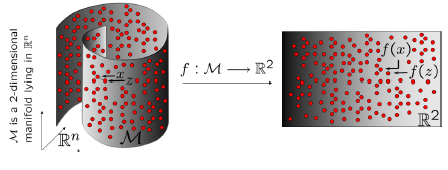
\includegraphics[width=\textwidth]{./Figures/manifold.png}
\caption{Manifold Learning \citep{Ety2008}}
\label{fig:manifold}
\end{center}
\end{figure}



\section{Motivation}
Consider the example of an image sequence. In the absence of features such as contour
points or wavelet coefficients, each image is a point in a space of dimension equal
to the number of image pixels. When facing an observation space of possibly tens or
hundreds of thousands of dimensions, it is often reasonable to assume that the data is not
dense in such a space and that many of the measured variables must be dependent with
only a few free parameters that are embedded in the observed variables, frequently in a
nonlinear way. Assuming that the number of free parameters remains the same throughout
the observations, and also assuming spatially smooth variation of the parameters,
we have geometric restrictions which can be well modeled as a manifold. Learning this manifold is a natural approach to the problem of modeling the data, with the advantage
of allowing nonlinear dimensionality reduction

\section{Contribution}
This paper presents a novel manifold learning approach for high dimensional
data, with emphasis on the problem of anomaly detection in image.

\section{Organization}




 

%----------------------------------------------------------------------------------------



%% Chapter 1
\chapter{Introduction} % Main chapter title

\label{Chapter1} % For referencing the chapter elsewhere, use \ref{Chapter1} 

\lhead{Chapter 1. \emph{Introduction}} % This is for the header on each page - perhaps a shortened title

%----------------------------------------------------------------------------------------
\section{Context}
\label{context}
The rapidly progressing digital revolution have infused enormous amount of images and video, which is growing constantly. Dealing with this large scale data calls for software application for enhancing image quality is the topic of Image Processing. Although image processing algorithms are getting accurate day by day, there is constant pressure on algorithms to deal with noise. It is inherent to the acquisition tools. State of the art preprocessing and postprocessing algorithms are being developed to suppress noise with altering the important content. The noise in an image is reduced by convolving the image with a Gaussian function. The above common approach blurs significant features and destroys some of the geometric information in the image \citep{Thor2009}. Image processing task are often tackled with geometric methods, which targets to understand the geometric configuration and relation between the observed objects. Manifold learning algorithms are one such geometric methods.

\section{Manifold Learning}
Manifold learning is form of unsupervised machine learning algorithms, which  extract low-dimensional structure from high dimensional data. These algorithms typically try to unfold the underlying manifold so that Euclidean distance in the new space is a meaningful measure of distance metrics between any pair of points. Manifold learning assumes that the data lies approximately on a low dimensional surface embedded in a high dimensional space \citep{Tal2008}. It can be further illustrated  using figure \ref{fig:manifold}, where manifold learning algorithms for non-linear data builds an embedding function $f$ mapping $\mathcal{M}$ to $\mathbb{R}^2$.

\begin{figure}[ht]
\begin{center}
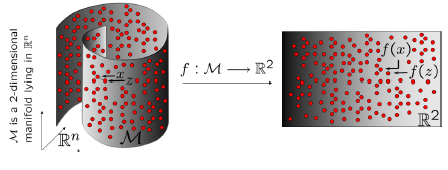
\includegraphics[width=\textwidth]{./Figures/manifold.png}
\caption{Manifold Learning \citep{Ety2008}}
\label{fig:manifold}
\end{center}
\end{figure}



\section{Motivation}
Consider the example of an image sequence. In the absence of features such as contour
points or wavelet coefficients, each image is a point in a space of dimension equal
to the number of image pixels. When facing an observation space of possibly tens or
hundreds of thousands of dimensions, it is often reasonable to assume that the data is not
dense in such a space and that many of the measured variables must be dependent with
only a few free parameters that are embedded in the observed variables, frequently in a
nonlinear way. Assuming that the number of free parameters remains the same throughout
the observations, and also assuming spatially smooth variation of the parameters,
we have geometric restrictions which can be well modeled as a manifold. Learning this manifold is a natural approach to the problem of modeling the data, with the advantage
of allowing nonlinear dimensionality reduction

\section{Contribution}
This paper presents a novel manifold learning approach for high dimensional
data, with emphasis on the problem of anomaly detection in image.

\section{Organization}




 

%----------------------------------------------------------------------------------------


 
%----------------------------------------------------------------------------------------
%	THESIS CONTENT - CHAPTER1
%----------------------------------------------------------------------------------------

%\mainmatter % Begin numeric (1,2,3...) page numbering

\pagestyle{fancy} % Return the page headers back to the "fancy" style

% Include the chapters of the thesis as separate files from the Chapters folder
% Uncomment the lines as you write the chapters

% Chapter 2
\chapter{Mathematical Background } % Main chapter title

\label{Chapter2} % For referencing the chapter elsewhere, use \ref{Chapter2} 

\lhead{Chapter 2. \emph{Mathematical Background}} % This is for the header on each page - perhaps a shortened title

%----------------------------------------------------------------------------
\section*{Overview}

This chapter is dedicated to provide mathematical notions necessary for under
standing the intuition behind manifold learning. Further, we present the
most representative manifold learning algorithms which are used in this thesis to solve specific problems in image processing and anomaly detection. We follow the structure from  Nicolas Thorstensen \citep{Thor2009} and Boothby \citep{Boot2003}. 
 
%----------------------------------------------------------------------------------------
\section{Metric Space}
Use of near and far is intuitive yet rigorous at the same time, which is rare in mathematics. Classifying the relationship between two 'primitives', whether they are close or far apart is some time not useful for the computation. A metric space is the mathematical construct of redefining the near and far primitive idea, which is useful in computation.


\begin{definition}

A metric on an arbitrary abstract set $\mathbb{X}$ is a function $d:\mathbb{X}\times \mathbb{X}\to [0,\infty)$ such that for all $a,b,c\in \mathbb{X}$, the following conditions are satisfied:

\begin{enumerate}
\item Non-negativity:	$d(a,b)\geq 0 and d(a,b)=0\Leftrightarrow a=b$
\item Symmetry:	$d(a,b)=d(b,a)$
\item Triangle inequality:  $d(a,c)\leq d(a,b)+d(b,c)$
	
\end{enumerate}

Then we say that $d$ is a \emph{metric} on $\mathbb{X}$ and that $(\mathbb{X},d)$ is a \emph{metric space}.

\end{definition}

A quite known instance of a metric space is the three dimensional
Euclidean space $\mathbb{R}^3$ with the Euclidean metric.


\begin{definition}\label{D;norm}
Let $V$ be a vector space over ${\mathbb R}$ and $N:V\rightarrow{\mathbb R}$ a map such that, $N({\mathbf v})=\|{\mathbf v}\|$, the following condition holds:
 
(i) Non-negativity: $\|{\mathbf v}\|\geq 0$ for all ${\mathbf v}\in V$. If $\|{\mathbf v}\|=0$, then ${\mathbf v}={\boldsymbol 0}$.

(ii) Linearity: If $\lambda\in{\mathbb R}$ and ${\mathbf v}\in V$,
then $\|\lambda{\mathbf v}\|=|\lambda| \|{\mathbf v}\|$.

(iii)Triangle inequality: If ${\mathbf v_1},\,{\mathbf v_2}\in V$, then 
$\|{\mathbf v_1}\|+\|{\mathbf v_2}\|\geq \|{\mathbf v_1}+{\mathbf v_2}\|$.

\noindent Then we call $\|\ \|$ a \emph{norm} and say that
$(V,\|\ \|)$ is a \emph{normed vector space}.
\end{definition}

Any normed vector space can be made into a metric space by the condition $d({\mathbf v_1},{\mathbf v_2})= \|{\mathbf v_1}-{\mathbf v_2}\|$.

\begin{definition}\label{D;inner product}
Let $V$ be a vector space over ${\mathbb R}$
and $M:V\times V\rightarrow{\mathbb R}$ a map such that,
writing $M({\mathbf v_1},{\mathbf v_2})
=\langle{\mathbf v_1},{\mathbf v_2}\rangle$, 
the following results
hold for ${\mathbf v_1},\,{\mathbf v_2},\,{\mathbf v_3}\in V$,
$\lambda\in{\mathbb R}$.

(i) $\langle{\mathbf v_1},{\mathbf v_2}\rangle\geq 0$.

(ii) If  $\langle{\mathbf v_1},{\mathbf v_2}\rangle=0$, then 
${\mathbf v_1}={\boldsymbol 0}$.

(iii)  $\langle{\mathbf v_1},{\mathbf v_2}\rangle
=\langle{\mathbf v_1},{\mathbf v_2}\rangle$.

(iv) $\langle{\mathbf v_1}+{\mathbf v_3},{\mathbf v_2}\rangle
=\langle{\mathbf v_1},{\mathbf v_2}\rangle
+\langle{\mathbf v_3},{\mathbf v_2}\rangle$.

(v) $\langle\lambda {\mathbf v_1},{\mathbf v_2}\rangle
=\lambda\langle{\mathbf v_1},{\mathbf v_2}\rangle$.

\noindent Then we call $\langle\ ,\  \rangle$ an 
\emph{inner product} and say that
$(V,\langle\ ,\  \rangle)$ is an \emph{inner product space}.
\end{definition}

Working on ${\mathbb R}^{n}$ to make it vector space, then 
$\langle{\mathbf x},{\mathbf y}\rangle=\sum_{j=1}^{n}x_{j}y_{j}$
is an inner product. We notice that the norm derived from inner product is called Euclidean norm.

\section{Topology}

With the metric structure in hand, the idea of 'near' and 'far' between elements of metric space can be quantified by characterizing the connectivity
of sets through small neighborhoods of elements which gives rise to a topology of the sets.

\begin{definition}
Let $(\mathbb{X},d)$ be a metric space and element $x \in \mathbb{X}$. If $r>0$, then $B_{open}(x,r)=\{y\,:\,d(x,y)<r\}$ is called as \emph{open ball} 
with centre ${\mathbf x}$ and radius $r$. Similarly, $B_{closed}(x,r)=\{y\,:\,d(x,y)\leq r\}$ is called closed ball.
\end{definition}

The topology of $\mathbb{X}$ induce by the
metric is easy to study. 

\begin{definition}\label{topology}
Let $\mathbb{X}$ be a set and $\tau$ a collection of subsets of $\mathbb{X}$ 
with the following properties.

(i) The empty set $\emptyset\in \tau$ and the space $\mathbb{X}\in\tau$.

(ii) If $U_{\alpha}\in\tau$ for all $\alpha\in A$, then
$\bigcup_{\alpha\in A} U_{\alpha}\in\tau$.

(iii) If $U_{j}\in\tau$ for all $1\leq j\leq n$, then
$\bigcap_{j=1}^{n} U_{j}\in\tau$.

Then we say that $\tau$ is a \emph{topology} on $\mathbb{X}$ and
that $(\mathbb{X},\tau)$ is a \emph{topological space}. 
\end{definition}

If $(\mathbb{X},d)$ is a metric space, then the collection of open sets forms a topology. The topology of a set allows one to study properties such as connectivity.

\subsection{Connectedness}

The metric space $(\mathbb{X}, d)$ is not connected if it is the union of two disjoint open nonempty sets. Similarly, the converse of earlier implies that $(\mathbb{X}, d)$ is connected. Mathematically, It can be defined as:

\begin{definition}\label{disconnected} 
A topological space $(\mathbb{X},\tau)$ is said to be \emph{disconnected} if we can find non-empty
open sets $V_1$ and $V_2$ such that $V_1\cup V_2=\mathbb{X}$
and $V_1\cap V_2=\emptyset$. A space which is not disconnected is called \emph{connected}.
\end{definition}

\subsection{Neighborhoods}

Hausdorff was the first one to define topologies in terms of neighborhoods. It always appears to be technically easier to define topologies in terms of open sets as we have been doing it so far. Generally, It can be defined as:
\begin{definition}\label{neighbourhood} 
Let $(\mathbb{X},\tau)$ be a topological space. If $x\in \mathbb{X}$, we say that $N$ is a \emph{neighbourhood} of $x$ if we can find $U\in\tau$ with $x\in U\subseteq N$.
\end{definition}

\section{Manifolds}
A manifold is a topological space that locally resembles Euclidean space near each point. More precisely, they are spaces that locally look like the much more familiar Euclidean spaces. This allows the well-understood notions on Euclidean spaces to be generalised to manifolds rather directly. Using all the above definition, we now define manifold.

\begin{definition}
A $d$-dimensional manifold is a topological space \ref{topology} in which 
points can be separated by neighborhoods \ref{neighbourhood} and where every point has a neighborhood that is homeomorphically mapped onto an open Euclidean ddimensional ball \citep{Thor2009}.
\end{definition}

As the general definition is not apt to perform vector calculus on a manifold, The the notion of a differentiable manifold comes hand in hand with the concept of coordinate chart \ref{chart}. It can be thought of as assigning a set of coordinates to the points in the neighborhood $U$.

\begin{figure}[ht]
\begin{center}
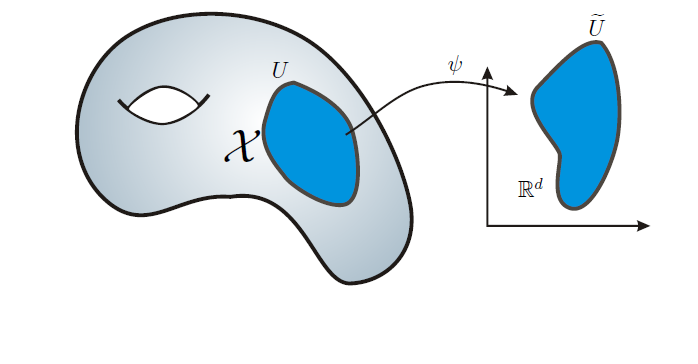
\includegraphics[width=\textwidth]{./Figures/chart.png}
\caption{Coordinate Chart\citep{Ety2008}}
\label{chart}
\end{center}
\end{figure}

To provide an entire description  of the manifold, several chart over manifold is used rather single. Transition map with two chart, corresponds to a change of coordinates is depicted in the figure \ref{TM}. 

\begin{figure}[ht]
\begin{center}
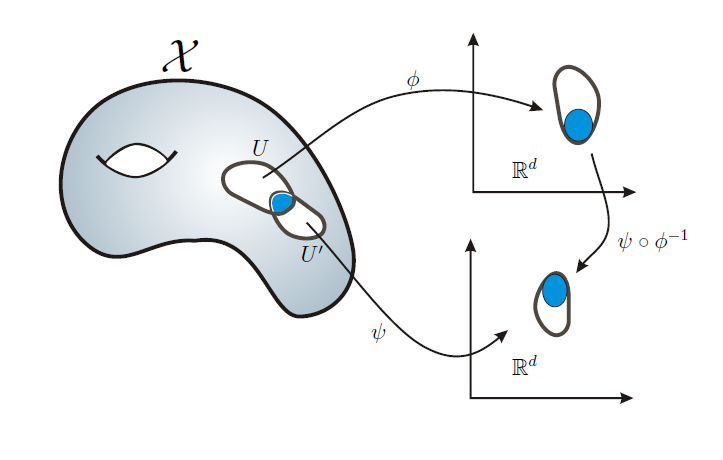
\includegraphics[width=\textwidth]{./Figures/TM.png}
\caption{Transition map.\citep{Ety2008}}
\label{TM}
\end{center}
\end{figure}

\section{Tangent Spaces}
The notion of linear approximation of a surface in vector calculus translates
to tangent space in differential geometry. The tangent space to a manifold $\mathcal{X}$ at a point $x$ is the closest flat approximation to $\mathcal{X}$ at that point.  If the dimension of $\mathcal{X}$ is $n$, then the tangent space is an $\mathbb{R}^n$ grazing $\mathcal{X}$ at $x$, as shown in figure \ref{tangent}. For detail discussion please refer work by Nicolas Thorstensen \citep{Thor2009} and Boothby \citep{Boot2003}.

\begin{figure}[ht]
\begin{center}
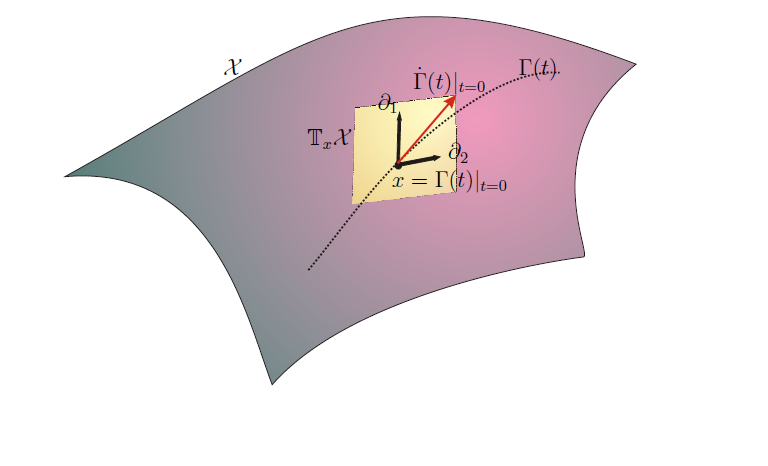
\includegraphics[width=\textwidth]{./Figures/tangent.png}
\caption{Tangent Space.\citep{Ety2008}}
\label{tangent}
\end{center}
\end{figure}

\subsection{Embedding}

When talking about the relationship between two topological objects, it is interesting to imagine a mapping from one object to the other that somehow preserves its original properties.

Let $\mathbb{X}$ and $\mathbb{Y}$ be two topological objects of the same type, a function $\phi \colon \mathbb{X} \to \mathbb{Y}$ is an embedding of $\mathbb{X}$ into $\mathbb{Y}$ if $\phi$ is an isomorphism which preserves the original properties of $\mathbb{X}$, where such properties are relative to the type of the objects at hand. Shortly, $\mathbb{X}$ is said to be \textit{embedded} in $\mathbb{Y}$.

\begin{example}[Embedding of Spaces]
	Consider the vector spaces $\mathbb{R}^p$ and $\mathbb{R}^q, p \leq q, p > 0$ and the isomorphism $t \colon \mathbb{R}^q \to \mathbb{R}^t \mid t(x) = [x | \bar{0}] = y$, where $y$ is the vector $x$ concatenated with $p-q$ zeros. $\mathbb{R}^p$ is embedded on $\mathbb{R}^q$, as the operations sum and scalar multiplication are preserved.
\end{example}

The same definition applies to manifolds too.
%% Chapter 2
\chapter{Mathematical Background } % Main chapter title

\label{Chapter2} % For referencing the chapter elsewhere, use \ref{Chapter2} 

\lhead{Chapter 2. \emph{Mathematical Background}} % This is for the header on each page - perhaps a shortened title

%----------------------------------------------------------------------------
\section*{Overview}

This chapter is dedicated to provide mathematical notions necessary for under
standing the intuition behind manifold learning. Further, we present the
most representative manifold learning algorithms which are used in this thesis to solve specific problems in image processing and anomaly detection. We follow the structure from  Nicolas Thorstensen \citep{Thor2009} and Boothby \citep{Boot2003}. 
 
%----------------------------------------------------------------------------------------
\section{Metric Space}
Use of near and far is intuitive yet rigorous at the same time, which is rare in mathematics. Classifying the relationship between two 'primitives', whether they are close or far apart is some time not useful for the computation. A metric space is the mathematical construct of redefining the near and far primitive idea, which is useful in computation.


\begin{definition}

A metric on an arbitrary abstract set $\mathbb{X}$ is a function $d:\mathbb{X}\times \mathbb{X}\to [0,\infty)$ such that for all $a,b,c\in \mathbb{X}$, the following conditions are satisfied:

\begin{enumerate}
\item Non-negativity:	$d(a,b)\geq 0 and d(a,b)=0\Leftrightarrow a=b$
\item Symmetry:	$d(a,b)=d(b,a)$
\item Triangle inequality:  $d(a,c)\leq d(a,b)+d(b,c)$
	
\end{enumerate}

Then we say that $d$ is a \emph{metric} on $\mathbb{X}$ and that $(\mathbb{X},d)$ is a \emph{metric space}.

\end{definition}

A quite known instance of a metric space is the three dimensional
Euclidean space $\mathbb{R}^3$ with the Euclidean metric.


\begin{definition}\label{D;norm}
Let $V$ be a vector space over ${\mathbb R}$ and $N:V\rightarrow{\mathbb R}$ a map such that, $N({\mathbf v})=\|{\mathbf v}\|$, the following condition holds:
 
(i) Non-negativity: $\|{\mathbf v}\|\geq 0$ for all ${\mathbf v}\in V$. If $\|{\mathbf v}\|=0$, then ${\mathbf v}={\boldsymbol 0}$.

(ii) Linearity: If $\lambda\in{\mathbb R}$ and ${\mathbf v}\in V$,
then $\|\lambda{\mathbf v}\|=|\lambda| \|{\mathbf v}\|$.

(iii)Triangle inequality: If ${\mathbf v_1},\,{\mathbf v_2}\in V$, then 
$\|{\mathbf v_1}\|+\|{\mathbf v_2}\|\geq \|{\mathbf v_1}+{\mathbf v_2}\|$.

\noindent Then we call $\|\ \|$ a \emph{norm} and say that
$(V,\|\ \|)$ is a \emph{normed vector space}.
\end{definition}

Any normed vector space can be made into a metric space by the condition $d({\mathbf v_1},{\mathbf v_2})= \|{\mathbf v_1}-{\mathbf v_2}\|$.

\begin{definition}\label{D;inner product}
Let $V$ be a vector space over ${\mathbb R}$
and $M:V\times V\rightarrow{\mathbb R}$ a map such that,
writing $M({\mathbf v_1},{\mathbf v_2})
=\langle{\mathbf v_1},{\mathbf v_2}\rangle$, 
the following results
hold for ${\mathbf v_1},\,{\mathbf v_2},\,{\mathbf v_3}\in V$,
$\lambda\in{\mathbb R}$.

(i) $\langle{\mathbf v_1},{\mathbf v_2}\rangle\geq 0$.

(ii) If  $\langle{\mathbf v_1},{\mathbf v_2}\rangle=0$, then 
${\mathbf v_1}={\boldsymbol 0}$.

(iii)  $\langle{\mathbf v_1},{\mathbf v_2}\rangle
=\langle{\mathbf v_1},{\mathbf v_2}\rangle$.

(iv) $\langle{\mathbf v_1}+{\mathbf v_3},{\mathbf v_2}\rangle
=\langle{\mathbf v_1},{\mathbf v_2}\rangle
+\langle{\mathbf v_3},{\mathbf v_2}\rangle$.

(v) $\langle\lambda {\mathbf v_1},{\mathbf v_2}\rangle
=\lambda\langle{\mathbf v_1},{\mathbf v_2}\rangle$.

\noindent Then we call $\langle\ ,\  \rangle$ an 
\emph{inner product} and say that
$(V,\langle\ ,\  \rangle)$ is an \emph{inner product space}.
\end{definition}

Working on ${\mathbb R}^{n}$ to make it vector space, then 
$\langle{\mathbf x},{\mathbf y}\rangle=\sum_{j=1}^{n}x_{j}y_{j}$
is an inner product. We notice that the norm derived from inner product is called Euclidean norm.

\section{Topology}

With the metric structure in hand, the idea of 'near' and 'far' between elements of metric space can be quantified by characterizing the connectivity
of sets through small neighborhoods of elements which gives rise to a topology of the sets.

\begin{definition}
Let $(\mathbb{X},d)$ be a metric space and element $x \in \mathbb{X}$. If $r>0$, then $B_{open}(x,r)=\{y\,:\,d(x,y)<r\}$ is called as \emph{open ball} 
with centre ${\mathbf x}$ and radius $r$. Similarly, $B_{closed}(x,r)=\{y\,:\,d(x,y)\leq r\}$ is called closed ball.
\end{definition}

The topology of $\mathbb{X}$ induce by the
metric is easy to study. 

\begin{definition}\label{topology}
Let $\mathbb{X}$ be a set and $\tau$ a collection of subsets of $\mathbb{X}$ 
with the following properties.

(i) The empty set $\emptyset\in \tau$ and the space $\mathbb{X}\in\tau$.

(ii) If $U_{\alpha}\in\tau$ for all $\alpha\in A$, then
$\bigcup_{\alpha\in A} U_{\alpha}\in\tau$.

(iii) If $U_{j}\in\tau$ for all $1\leq j\leq n$, then
$\bigcap_{j=1}^{n} U_{j}\in\tau$.

Then we say that $\tau$ is a \emph{topology} on $\mathbb{X}$ and
that $(\mathbb{X},\tau)$ is a \emph{topological space}. 
\end{definition}

If $(\mathbb{X},d)$ is a metric space, then the collection of open sets forms a topology. The topology of a set allows one to study properties such as connectivity.

\subsection{Connectedness}

The metric space $(\mathbb{X}, d)$ is not connected if it is the union of two disjoint open nonempty sets. Similarly, the converse of earlier implies that $(\mathbb{X}, d)$ is connected. Mathematically, It can be defined as:

\begin{definition}\label{disconnected} 
A topological space $(\mathbb{X},\tau)$ is said to be \emph{disconnected} if we can find non-empty
open sets $V_1$ and $V_2$ such that $V_1\cup V_2=\mathbb{X}$
and $V_1\cap V_2=\emptyset$. A space which is not disconnected is called \emph{connected}.
\end{definition}

\subsection{Neighborhoods}

Hausdorff was the first one to define topologies in terms of neighborhoods. It always appears to be technically easier to define topologies in terms of open sets as we have been doing it so far. Generally, It can be defined as:
\begin{definition}\label{neighbourhood} 
Let $(\mathbb{X},\tau)$ be a topological space. If $x\in \mathbb{X}$, we say that $N$ is a \emph{neighbourhood} of $x$ if we can find $U\in\tau$ with $x\in U\subseteq N$.
\end{definition}

\section{Manifolds}
A manifold is a topological space that locally resembles Euclidean space near each point. More precisely, they are spaces that locally look like the much more familiar Euclidean spaces. This allows the well-understood notions on Euclidean spaces to be generalised to manifolds rather directly. Using all the above definition, we now define manifold.

\begin{definition}
A $d$-dimensional manifold is a topological space \ref{topology} in which 
points can be separated by neighborhoods \ref{neighbourhood} and where every point has a neighborhood that is homeomorphically mapped onto an open Euclidean ddimensional ball \citep{Thor2009}.
\end{definition}

As the general definition is not apt to perform vector calculus on a manifold, The the notion of a differentiable manifold comes hand in hand with the concept of coordinate chart \ref{chart}. It can be thought of as assigning a set of coordinates to the points in the neighborhood $U$.

\begin{figure}[ht]
\begin{center}
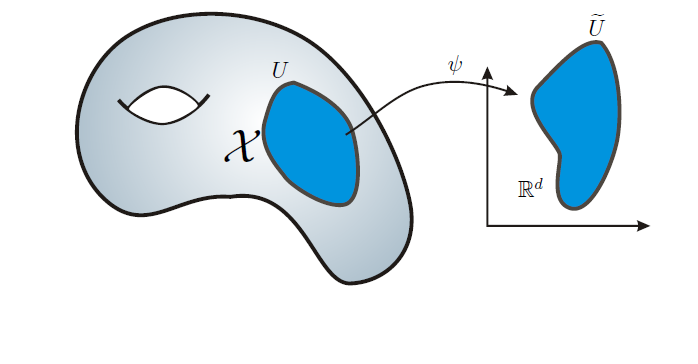
\includegraphics[width=\textwidth]{./Figures/chart.png}
\caption{Coordinate Chart\citep{Ety2008}}
\label{chart}
\end{center}
\end{figure}

To provide an entire description  of the manifold, several chart over manifold is used rather single. Transition map with two chart, corresponds to a change of coordinates is depicted in the figure \ref{TM}. 

\begin{figure}[ht]
\begin{center}
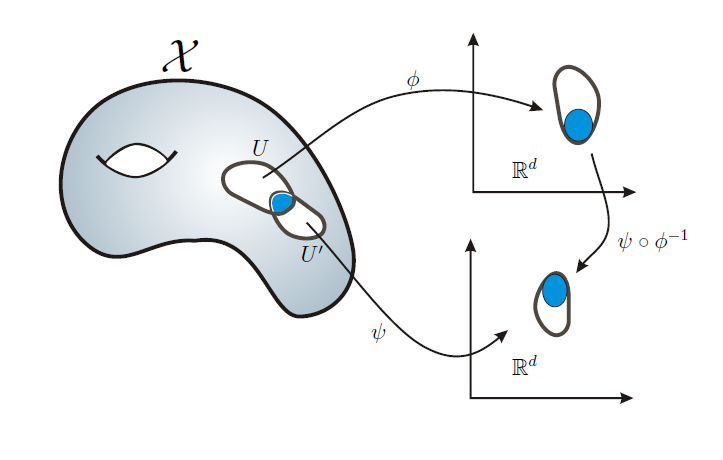
\includegraphics[width=\textwidth]{./Figures/TM.png}
\caption{Transition map.\citep{Ety2008}}
\label{TM}
\end{center}
\end{figure}

\section{Tangent Spaces}
The notion of linear approximation of a surface in vector calculus translates
to tangent space in differential geometry. The tangent space to a manifold $\mathcal{X}$ at a point $x$ is the closest flat approximation to $\mathcal{X}$ at that point.  If the dimension of $\mathcal{X}$ is $n$, then the tangent space is an $\mathbb{R}^n$ grazing $\mathcal{X}$ at $x$, as shown in figure \ref{tangent}. For detail discussion please refer work by Nicolas Thorstensen \citep{Thor2009} and Boothby \citep{Boot2003}.

\begin{figure}[ht]
\begin{center}
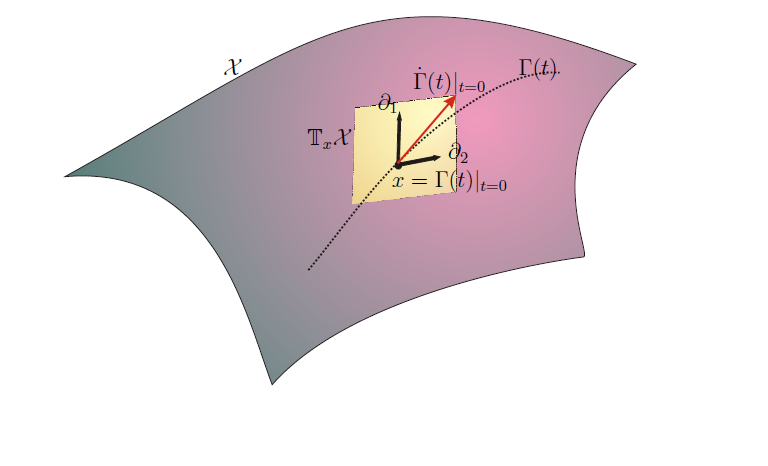
\includegraphics[width=\textwidth]{./Figures/tangent.png}
\caption{Tangent Space.\citep{Ety2008}}
\label{tangent}
\end{center}
\end{figure}

\subsection{Embedding}

When talking about the relationship between two topological objects, it is interesting to imagine a mapping from one object to the other that somehow preserves its original properties.

Let $\mathbb{X}$ and $\mathbb{Y}$ be two topological objects of the same type, a function $\phi \colon \mathbb{X} \to \mathbb{Y}$ is an embedding of $\mathbb{X}$ into $\mathbb{Y}$ if $\phi$ is an isomorphism which preserves the original properties of $\mathbb{X}$, where such properties are relative to the type of the objects at hand. Shortly, $\mathbb{X}$ is said to be \textit{embedded} in $\mathbb{Y}$.

\begin{example}[Embedding of Spaces]
	Consider the vector spaces $\mathbb{R}^p$ and $\mathbb{R}^q, p \leq q, p > 0$ and the isomorphism $t \colon \mathbb{R}^q \to \mathbb{R}^t \mid t(x) = [x | \bar{0}] = y$, where $y$ is the vector $x$ concatenated with $p-q$ zeros. $\mathbb{R}^p$ is embedded on $\mathbb{R}^q$, as the operations sum and scalar multiplication are preserved.
\end{example}

The same definition applies to manifolds too. 
%----------------------------------------------------------------------------------------
%	THESIS CONTENT - CHAPTER2
%----------------------------------------------------------------------------------------

%\mainmatter % Begin numeric (1,2,3...) page numbering

\pagestyle{fancy} % Return the page headers back to the "fancy" style

% Include the chapters of the thesis as separate files from the Chapters folder
% Uncomment the lines as you write the chapters

% Chapter 3
\chapter{Manifold Learning} % Main chapter title

\label{Chapter3} % For referencing the chapter elsewhere, use \ref{Chapter1} 

\lhead{Chapter3. \emph{Manifold Learning}} % This is for the header on each page - perhaps a shortened title

%-------------------------------------------------------------------------------
\section*{Overview}
Manifold learning is an emerging and promising approach in nonparametric dimension reduction widely used in image processing, data mining, signals processing and computer vision. The core theme of manifold leaning is to find the most succinct low dimensional structure that is embedded
in a higher dimensional space. Using earlier, the algorithms can work directly in the lower dimensional latent space of the manifold rather high dimensional data space and thus get computationally efficient. In this chapter, we review the representative sample of manifold learning, mathematical developments, as well as some interesting applications. 
%----------------------------------------------------------------------------------------
\section{Introduction}
Most of the datasets encountered in image processing often consist of
a large number of samples each of which are themselves of high dimension.
Further processing of the datum is done either treating it directly or extracting complex features before processing. Nevertheless, it  wither its
entire datum or a set extracted features, the dimensionality of
problems usually remain high. This in turn slows down the processing considerably or sometimes making the treatment even intractable. The task to reducing the computational burden is to reduce the dimensionality of the data. Dimensionality reduction can be thought of as mathematical mapping of high-dimensional data into a meaningful representation of the intrinsic dimensionality. The intrinsic dimensionality of a data set can be defined as the lowest number of variables that can preserve the geometrical structure of the data.


\section{Problem Definition}
Given a set of of high-dimensional training instances $\mathbb{X} = \{x_1, x_2, ...,x_N \}$, where $x_{i} \in \mathbb{R}^D$. We assume that $\mathbb{X}$ approximately lie on a smooth manifold $\mathcal{X}$. The idea of manifold learning algorithms is to find an embedding set $\mathbb{Y} = \{y_1, y_2, ...,y_N \} $ of $\mathbb{X}$ in low dimension space $\mathbb{R}^d$, where $d<D$. The local manifold structure formed by $\mathbb{X}$ in the original space $\mathbb{R}^D$ is preserved in the embedded space $\mathbb{R}^d$.


Manifold Learning can be mainly divided into linear and non linear methods.
Linear methods, which have long been used for analyzing multivariate data, include principal component analysis (PCA) and multidimensional scaling (MDS). A further distinction within non-linear methods is to divide the methods into two classes: one is to preserve the global geometric structure of manifold, such as Isomap \citep{Tene2000} and the other one is to preserve the local neighborhood geometric structure, such as LLE \citep{Roweis2000}.

\section{Linear Methods}
\subsection{Principle Component Analysis}
\label{s:pca}

Principal component analysis (PCA) is a standard algorithm to explain the dispersion of a point cloud by projecting data onto a carefully chosen linear subspace. It reduces the dimensionality of the point cloud while keeping the maximum of variance information. The dispersion in linear subspaces of higher dimension is captured by by building an orthonormal basis such that the projection along each axis has a decreasing maximum variance. 

We consider n points $\mathbf{X} = \{x_1, x_2, ..., x_n\}$ of dimension D from $\mathbb{R}^D$. Also, let us assume $V^{*}$ be a d-dimensional subspace of $\mathbb{R}^D$ and let $ u = \{u_1, u_2, ..., u_D\}$ be an orthonormal basis of $\mathbb{R}^D$ such that $\{u_1, u_2, ..., u_d\}$ is a basis of V. Then each data point is approximated by:

\begin{equation}
y_n = \sum_{i=1}^{d} a_{n,i}u_{i} + \sum_{i=1}^{D+1} a_{n,i}u_{i}
\end{equation}

The below energy function is used to recover $u_1, u_3, ..., u_d$.
\begin{equation}
\mathbb{E} = \frac{1}{N}\sum_{n=1}^{N} \|x_n - y_n\|^{2}
\end{equation}

This is equivalent to minimizing the approximation error. 

\begin{equation}
x_n - y_n = \sum_{i=d+1}^{D} \{(x_n - \bar{x})^T u_i\}u_i
\label{p_3}
\end{equation} 
The above equation \ref{p_3} can be best visualized in the figure \ref{pca}.

\begin{figure}[ht]
\begin{center}
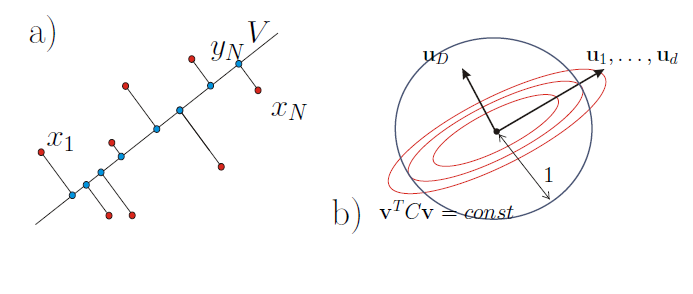
\includegraphics[width=\textwidth]{./Figures/pca.png}
\caption{a) Manifold with original (red) and projected (blue) points. b) Geometry and constraint visualization of optimization function. Pictures taken from Nicolas Thorstensen works \citep{Ety2008}}
\label{pca}
\end{center}
\end{figure}

Now, we can write the energy function as
\begin{equation}
\mathbb{E} = \frac{1}{N}\sum_{n=1}^{N}\sum_{i=d+1}^{D} (x_n^{T}u_{i}- \bar{x}^{T}u_i)^2 = \sum_{i=d+1}^{D}u_{i}^{T}\mathbf{C}u_{i}
\end{equation}

$\mathbf{C}$ is defined as covariance matrix, $\mathbf{C} = \frac{1}{N}\sum_{n=1}^{N}(x_n-\bar{x})(x_n -\bar{x})^2$. Our optimization problem look like
\begin{equation}
\begin{aligned}
& \underset{D}{\text{minimize}}
&& \mathbb{E} = u_{D}^{T}\mathbf{C}u_{D} \\
& \text{subject to}
&& u_{D}^{T}u_{D} = 1
\end{aligned}
\end{equation}
Now using Lagrange multipliers, we solve this constraint optimization problem as
\begin{equation}
u_{D}^{T}\mathbf{C}u_{D}+\lambda(1-u_{D}^{T}u_{D})=0
\label{LM}
\end{equation}

The solution off the above equation gives standard form eigenvalue problem $\mathbf{C}u_D =\lambda u_D$. The geometry of the minimization problem is illustrated in figure \ref{pca} b).

We take an input image \ref{app_pca} (A), which is sequence of vector in $\mathbb{R}^{4096}$ representing the brightness values of $64\times64$ pixel image of the face. The 1st dimension representing embedding correlates with intrinsic-dimension of one, which is left-right pose. The two-dimensional projection of original input image found by PCA is shown in figure \ref{app_pca} (B).

\begin{figure}
\centering
\begin{subfigure}{.5\textwidth}
  \centering
  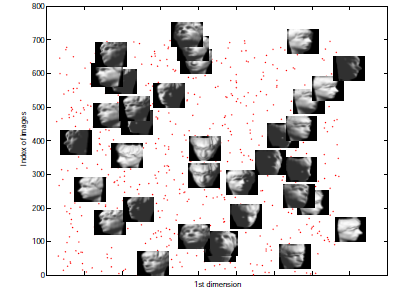
\includegraphics[width=\linewidth]{./Figures/original.png}
\caption{Input}
%  \label{fig:sub1}
\end{subfigure}%
\begin{subfigure}{.5\textwidth}
  \centering
  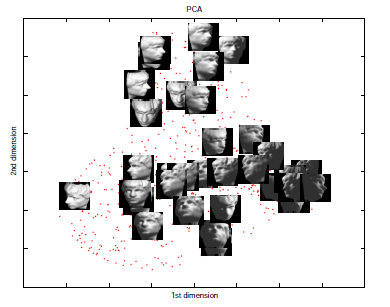
\includegraphics[width=\linewidth]{./Figures/o_pca.png}
  \caption{Output}
%  \label{fig:sub2}
\end{subfigure}
\caption{Application of PCA. }
\label{app_pca}
\end{figure}

\subsection{Multi-Dimensional Scaling}
\label{s:MDS}

The Multi-Dimensional Scaling (MDS), is a PCA-like technique that maps the original high dimensional space to a lower dimensional space by preserving pairwise distances. Figure \ref{app_mds} shows an example of MDS, where pairwise distance is preserved. MDS \citep{Cox2000} is applied when it difficult to calculate   covariance matrix from the dataset, when data are, for instance, qualitative or infinite dimensional, when only a point-wise distance is known or also when the size $\mathbb{D}$ of the sample set is lower than the dimension of data \citep{Ety2008}.


MDS addresses the problem of finding d-dimensional Euclidean coordinates
for each data sample ($x_i \in \mathbf{X}$) so that the pairwise distance ($d$) of their Euclidean coordinates match the original pairwise distance as closely as possible. 

We define $N \times N$ euclidean distance or affinity matrices $\mathbf{D}$ as symmetric, $d_{ii}=0$ and $d_{ij}>0$, if $i \neq j$. With $\mathbf{D}$ matrix in hand, the MDS algorithm attempts to find $N$ data points $\mathbf{Y} = y_1, y_2, y_3,...,y_N$ in $\mathbb{R}^d$ such that distance matrix is preserved as depicted in the figure \ref{mds}.


\begin{figure}
\centering
\begin{subfigure}{.5\textwidth}
  \centering
  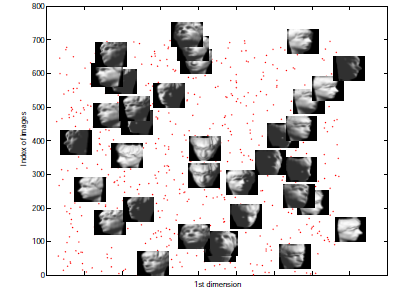
\includegraphics[width=\linewidth]{./Figures/original.png}
\caption{Input}
%  \label{fig:sub1}
\end{subfigure}%
\begin{subfigure}{.5\textwidth}
  \centering
  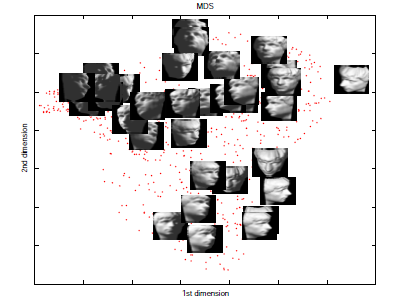
\includegraphics[width=\linewidth]{./Figures/o_mds.png}
  \caption{Output}
%  \label{fig:sub2}
\end{subfigure}
\caption{Application of MDS.}
\label{app_mds}
\end{figure}

\begin{figure}[ht]
\begin{center}
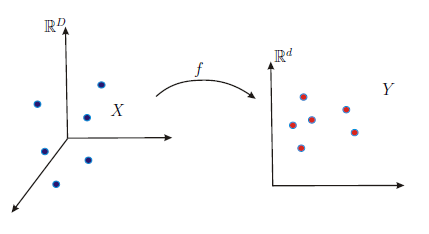
\includegraphics[width=\textwidth]{./Figures/mds.png}
\caption {Multi-Dimensional Scaling}
\label{mds}
\end{center}
\end{figure}

In particular, we try to optimize following function:

\begin{equation}
\begin{aligned}
& \underset{\mathbf{Y}}{\text{Min}}
&& \sum_{i=1}^{N}\sum_{i=1}^{N}(d_{ij}^{\mathbf{X}}-d_{ij}^{\mathbf{Y}})^{2}
\label{mds:1}
\end{aligned}
\end{equation}

where, $d_{ij}^{\mathbf{X}}$ and $d_{ij}^{\mathbf{Y}}$ is normed distance from sample point $x_{i}$ and $x_{i}$ respectively. Converting distance $\mathbf{D}^{\mathbb{X}}$ matrix into kernel matrix of inner product yields:

\begin{equation}
\mathbf{X}^{T}\mathbf{X} = -\frac{1}{2}\mathbf{J}\mathbf{D}^{\mathbb{X}}
\end{equation}
where $\mathbf{J} = \mathcal{I}d_{N}-\frac{1}{N}\mathbf{1}\mathbf{1}^{T}$. Now the equation \ref{mds:1} can be reduced into

\begin{equation}
\begin{aligned}
& \underset{\mathbf{Y}}{\text{Min}}
&& \sum_{i=1}^{N}\sum_{i=1}^{N}(x_{i}^{T}x_{j}-y_{i}^{T}y_{j})^{2}
\label{mds:2}
\end{aligned}
\end{equation}


Solving equation \ref{mds:2} as shown in Cox and Cox paper\citep{Cox2000} gives $\mathbf{Y}=\lambda^{\frac{1}{2}}\mathbf{U}^{T}$. Here, $\mathbf{U}$ is eigenvector of $\mathbf{X}^{T}\mathbf{X}$ corresponding to top d eigenvalues, and $\lambda$ is top d eigenvalues of $\mathbf{X}^{T}\mathbf{X}$.


MDS can be generalized into to geodesic distances between point samples from
a non-linear manifold. But a non-convex energy function coming out makes it  
tedious to optimize. In the next section we will provide an overview of non-linear manifold algorithms.


\section{Non-Linear Methods}

Linear methods such as PCA and MDS fails to produce desired results when the data is sampled from non linear manifolds \citep{Thor2009}. We now review representative non-linear methods in manifold learning in this section with assumption that the data is distributed along a d-dimensional submanifold $\mathcal{X}$ embedded in $\mathbb{R}^{D}$.

\subsection{Graph-based Algorithms}

Manifold learning based on graph based algorithms often relies on preserving the geometric structure in the neighborhood of some points. The important step is to construct a graph using $K$-nearest neighbor graph or $\epsilon$-neighborhood and apply MDS as previously detailed.

\subsubsection{Isomap}
\label{s:isomap}

Isomap was proposed by Joshua Tenenbaum, Vin de Silva and John Langford in Science \citep{Tene2000}. It is an extended version of MDS for data lying on smooth non-linear manifold. Unlike MDS, the pairwise distance matrix in Isomap is replaced by the matrix of pairwise geodesic distances approximated by distances in graphs. The algorithm proceeds in three steps. First a distance $d(x; y)$ is considered in the data space. Then, a neighborhood graph based on a $\epsilon$-neighborhood or $k$-nearest neighbor points is build with following weights $D_{ij} = d(xi; xj)$ if an edge link
exists between points $x_i$ and $x_j$ , otherwise $D_{ij} = 1$. The pairwise distance matrix $\mathbf{D}$ is then calculated using a Dijkstra-like algorithm in the graph. Finally, the data via MDS is embedded so as to preserve these distances. A two-dimensional projection using isomap is shown in the figure \ref{app_iso} with k=6.

\begin{figure}
\centering
\begin{subfigure}{.5\textwidth}
  \centering
  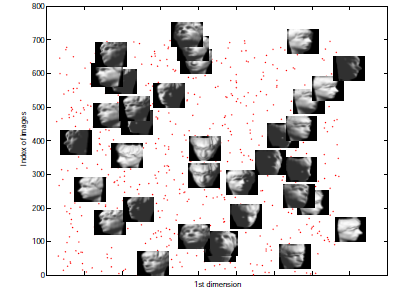
\includegraphics[width=\linewidth]{./Figures/original.png}
\caption{Input}
%  \label{fig:sub1}
\end{subfigure}%
\begin{subfigure}{.5\textwidth}
  \centering
  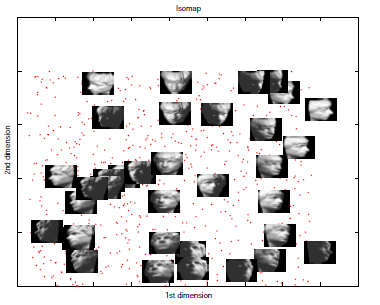
\includegraphics[width=\linewidth]{./Figures/o_iso.png}
  \caption{Output}
%  \label{fig:sub2}
\end{subfigure}
\caption{Application of Isomap}
\label{app_iso}
\end{figure}

Precautionary measure should be taken while calculating distances between far apart points on the manifold, which can be very close in the data space as discussed in the figure \ref{isomap}.
\begin{figure}[ht]
\begin{center}
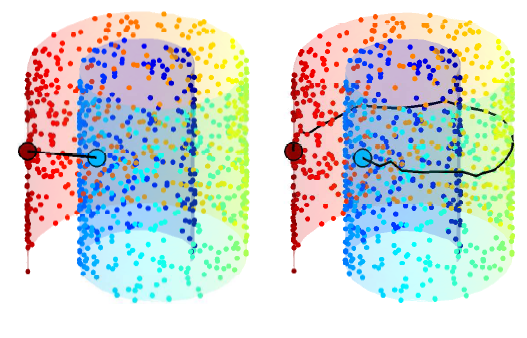
\includegraphics[width=\textwidth]{./Figures/isomap.png}
\caption {Multi-Dimensional Scaling. Left: Distance between two
points using a distance in the data space. Right: Distance between two points
using an approximated geodesic path. Image taken from Patrick Etyngier work \citep{Ety2008}.}
\label{isomap}
\end{center}
\end{figure}

\subsubsection{Locally linear Embedding}
\label{s:lle}
Locally linear Embedding (LLE) is a manifold mapping dimension reduction algorithm introduced by Roweis \& Saul \citep{Roweis2000}. It aims at recovering the low dimensional geometry of the data by looking at the local interaction between data points. The construction of a nearest neighbor graph recovers the local interactions. Then further processing is done to reduce the dimensionality of the data and provide a parametrization in a d- dimensional hyperplane. LLE algorithm can be summarized in the following steps:

\begin{enumerate}
\item  Neighborhood graph $\mathcal{G}$ is build on the dataset $\mathbb{X}$ using K-nearest neighbour method. 
\item Weights $W_{ij}$ are calculated to each of the nearest neighbours pair $(x_i, y_i)$ by minimising the cost function:
      \begin{equation}
     \epsilon(W) = \sum_{i}\vert x_{i} - \sum_{j=1}^k W_{ij} x_{j}\vert^{2}
    \end{equation}
   
\item The inner products between each point $x_i$ and each of its nearest neighbours are computed to produce gram positive-semidefinite matrix, $G_{jk} = (x -x_j)^T(x-x_i)$.
\item  The reconstruction weights are then computed using:
    \begin{equation}
     W_{ij} = \sum_{k}\mathbb{G}-{jk}^{-1}(G_{jk}+\lambda)
    \end{equation}
    such that, $W_{ij} =0 $ if $x_{j}$ is not one of the nearest neighbours of $x_{i}$ and $\sum_{j} W_{ij} = 1$)
    
\item Finally the embedded $\mathbb{Y}$ which will make up the final output data are calculated by minimising a second cost function:
    \begin{equation}
     \Phi(Y) = \sum_{i}\vert y_{i}-\sum_{j}W_{ij}y_{j}\vert^{2}
    \end{equation}
We also constraint $\sum_{i}y_{i} = 0$ to centre the projection on the origin. The other constraint is imposed in order to avoid degenerate solutions;
    \begin{equation}
     \frac{1}{n}\sum_{i}y_{i}y_{i}^{T} = I
    \end{equation}
    where I is the d$\times$d identity matrix.
    
\item     This cost function now defines a quadratic form containing the N$\times$N symmetric matrix $M_{ij}$:
    \begin{equation}
     \Phi(I) =\sum_{ij}M_{ij}y_{i}y_{i}^{T}
    \end{equation}
    where $M_{ij} = \delta_{ij}-W_{ij}-W_{ij}+\sum_{k}W_{ki}W_{kj}$ and $\delta_{ij} = 1$ if $i = j$ and $\delta_{ij} = 0$ otherwise.
\item The embedding $\mathbb{Y}$ is then given by the the lowest d+1 eigenvectors of the matrix $M_{ij}$. The bottom eigenvector representing a 
free translation mode of eigenvalue 0 is left out in order to find the optimum embedding.

\end{enumerate}

The geometry the optimization problem is depicted in figure \ref{lle}.

\begin{figure}[ht]
\begin{center}
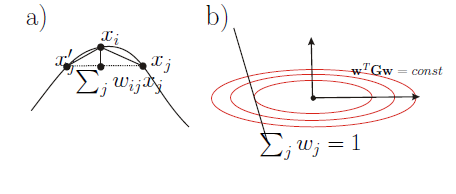
\includegraphics[width=\textwidth]{./Figures/lle.png}
\caption {LLE. a) $x_i$ is appropriated by its neighborhood $(x_{j}^{'}, x_{j})$. b) The black line touching the level set at a single point defines the constraints}
\label{lle} 
\end{center}
\end{figure}

A two-dimensional projection of the original input by using with k=5 is shown in the figure \ref{app_lle}.
\begin{figure}
\centering
\begin{subfigure}{.5\textwidth}
  \centering
  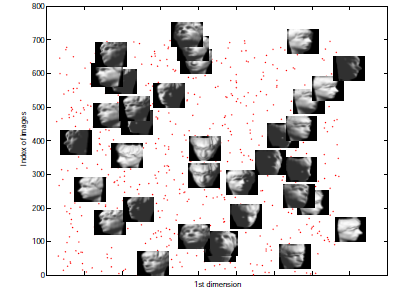
\includegraphics[width=\linewidth]{./Figures/original.png}
\caption{Input}
%  \label{fig:sub1}
\end{subfigure}%
\begin{subfigure}{.5\textwidth}
  \centering
  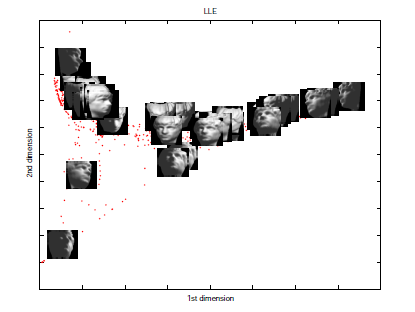
\includegraphics[width=\linewidth]{./Figures/o_lle.png}
  \caption{Output}
%  \label{fig:sub2}
\end{subfigure}
\caption{Application of LLE}
\label{app_lle}
\end{figure}

\subsection{Laplacian-based Algorithms}
Laplacian based algorithms assume that data have a structure of low dimensional manifold embedded in a higher dimensional space. The maps are constructed into a low dimensional space preserving the local neighborhood topology. In this part, we give outlines of representative laplacian based algorithms.

\subsubsection{Laplacian Eigenmaps}
\label{s:le}
Laplacian Eigenmaps were introduced by Belkin \citep{Bel2002}. Its intent is
to embed the observed data $\mathbf{X}$ into $\mathbb{R}^d$ by first constructing the $k$-nearest-neighbor or $\epsilon$-graph $\mathcal{G}$ from $\mathbf{X}$. In the $k$-nearest-neighbor graph, an edge is present between $x_i$ and $x_j$ if $x_i$ is among the $k$ nearest neighbors of $x_j$ or vice versa. In the $\epsilon$-graph, $x_i$ and $x_j$ are adjacent if $\|x_i-x_j\|^2<\epsilon$ for a given threshold parameter $\epsilon$. The weighted adjacency matrix of $\mathcal{G}$ is defined as $\mathbf{W}$, $$\mathbf{W}_{ij}=\begin{cases} \mathbf{K}_{ij} &\mbox{ if } \{i,j\}\in E\\
                0 &\mbox{ else}, \end{cases}$$ and let $\mathbf{D}\in\mathbb{R}^{N\times N}$ be the diagonal matrix defined by $\mathbf{D}_{ii}=\sum_{j}\mathbf{W}_{ij}$ for $i\in[N]$.
                
Then the normalized weighted graph Laplacian of $\mathbf{G}$ \citep{Bel2002}
is given by $\mathbf{W}=\mathbf{D}^{-1/2}\mathbf{W}\mathbf{D}^{-1/2}$.
If we represent eigendecomposition of $\mathbf{W}$  by $\mathbf{W}=\mathbf{U}\Lambda \mathbf{U}^\top$ with the diagonal entries of $\Lambda$ non-increasing, then Laplacian eigenmaps embeds $\mathbf{X}$ via
$\mathbf{U}[:,2:d+1]$---the first $d$ nontrivial eigenvectors of $\mathbf{W}$. The local geometry of $\mathbf{X}$ is optimally preserved in a least squares sense by the former.
 
A two-dimensional projection of the original input by using with k=9 is shown in the figure \ref{app_le}.
 
\begin{figure}
\centering
\begin{subfigure}{.5\textwidth}
  \centering
  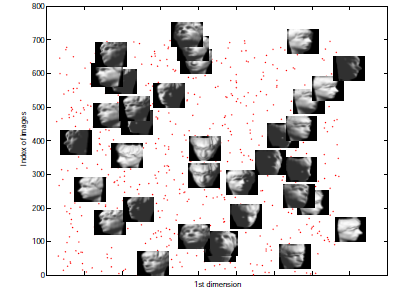
\includegraphics[width=\linewidth]{./Figures/original.png}
\caption{Input}
%  \label{fig:sub1}
\end{subfigure}%
\begin{subfigure}{.5\textwidth}
  \centering
  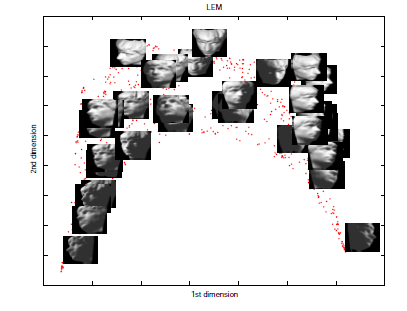
\includegraphics[width=\linewidth]{./Figures/o_le.png}
  \caption{Output}
%  \label{fig:sub2}
\end{subfigure}
\caption{Application of Laplacian Eigenmaps}
\label{app_le}
\end{figure}



\subsubsection{Diffusion Maps}
\label{s:dm}

The objective of Diffusion Maps (DM) is to define a metric, named the diffusion distance, that measures the connectivity between points in an arbitrary set. We will follow the construction of DM as described
in the paper by Lindenbaum and others \citep{Lind2015}.

Representing the high dimensional input dataset \begin{math} \mymat{X} \end{math}, the DM framework contains the following steps:

\begin{enumerate}

\item A kernel function  \begin{math}{{\cal{K}} : \mymat{X}\times{\mymat{X}}\longrightarrow{\mathbb{R}}  }
	\end{math} is chosen to define an anisotropic transition matrix, represented by $\mymat{K} \in {\mathbb{R}^{D \times D}}$. It satisfies the following properties for all 
	\begin{math}{(\myvec{x}_i,\myvec{x}_j) \in {\mymat{X}} }
	\end{math}.
	
	\begin{enumerate}
	
     \item Symmetry: \begin{math}{K_{i,j}={\cal{K}}(\myvec{x}_i,\myvec{x}_j)={\cal{K}}(\myvec{x}_j,\myvec{x}_i) }
	\end{math}, 
	
	\item Positive semi-definiteness: \begin{math}{ \myvec{v}_i^T  \mymat{K}  \myvec{v}_i \geq 0 }\end{math} for all $\myvec{v}_i \in
	\mathbb{R}^D$ and 
	
	\item Non-Negativity \begin{math}{{\cal{K}}(\myvec{x}_i,\myvec{x}_j)
		\geq 0. }
	\end{math}
	\end{enumerate}
	
\item {When we normalize the kernel using  $\mymat{M}$; where  \begin{math} M_{i,i}=\underset{j}{\sum}{K_{i,j}} \end{math}, the following matrix elements are computed:  
\begin{equation}
		{P_{i,j}^x={\cal{P}}(\myvec{x}_i,\myvec{x}_j)=[{{\mymat{M}}^{-1}{\mymat{K}}  }}]_{i,j}
		\label{EquationPDM}
		.\end{equation}
		
		 The resulting matrix $ \mymat{P}^x \in \mathbb{R}^{D
			\times D} $ is actually transition kernel of a 
		Markov chain on $\mymat{X}$ such that the expression
		${[{(\mymat{P}^x)^t}]_{i,j}}=p_t(\myvec{x}_i$,$\myvec{x}_j)$
		describes the transition probability from point
		\begin{math}{\myvec{x}_i}
		\end{math} to point \begin{math}{\myvec{x}_j}
		\end{math} in $t$ steps.
	}
\item{ Next, the spectral decomposition is applied to matrix \begin{math}  \mymat{P}^x \end{math} to obtain a sequence of eigenvalues  \begin{math}{\lbrace {\lambda_d}\rbrace }
		\end{math} and normalized eigenvectors \begin{math}{\lbrace{{\mbox{\boldmath${\psi}$}}_d}\rbrace }
		\end{math} that satisfies ${ {\mymat{P}^x}  {\mbox{\boldmath${\psi}$}_d} =\lambda_m{\mbox{\boldmath${\psi}$}}_d, d=0,...,D-1}
		$; }
\item{
		Defining a new representation for the dataset $\mymat{X}$
		\begin{equation}{ \myvec{\Psi}_t{(\myvec{x}_i)}:   \myvec{x}_i
			\longmapsto \begin{bmatrix} { \lambda_1^{t}\psi_1[i]} , {
				\lambda_2^{t}\psi_2[i]} , { \lambda_3^{t}\psi_3[i]} , {.} {.} {.}
			,
			
			{\lambda_{D-1}^{t}\psi_{D-1}[i]}\\
			
			\end{bmatrix}^T \in{\mathbb{R}^{D-1}} },
		\end{equation}
		where $t$ is the selected number of steps and $\psi_d[i]$ denotes the $i^{\rm{th}}$ element of ${\mbox{\boldmath${\psi}$}_d}$.
		
Now the Euclidian distance between two data points is equal to the weighted $L_2$ distance between the conditional probabilities ${{p}_t(\myvec{x}_i,:)}$, and ${{p}_t(\myvec{x}_j,:)}$, $i,j=1,...,D$ (the $i$-th and $j$-th rows of $\myvec{P}^t$), which is referred as the Diffusion Distance
			\begin{equation}{ \label{EqDist} { {\cal{D}}^2_t( \myvec{x}_i,\myvec{x}_j)=||{\mymat{\Psi}_t{(\myvec{x}_i)}}-{\mymat{\Psi}_t{(\myvec{x}_j)}}||^2={  \sum_{d\geq{1}} {\lambda}^{2t}_d (\psi_d[i]-\psi_d[j])^2 }}=\\
			||{p_t}(\myvec{x}_i,:)-{p_t}(\myvec{x}_j,:)||^2_{\tiny\mymat{W}^{-1}}},
			\end{equation}
			where $\mymat{W}$ is a diagonal matrix with elements
			$W_{i,i}=\frac{D_{i,i}}{\sum_{i=1}^M D_{i,i}}$.}
	\item{The desired accuracy $\delta \geq 0$ is chosen for the diffusion distance defined by Eq. (\ref{EqDist}) such that
		$s(\delta,t)=\text{max} \{\ell\in \mathbb{N}$  such that   $|\lambda_{\ell}|^t > \delta |\lambda_1|^t \}  $. By using $\delta$, a new mapping
		of $s(\delta,t)$ dimensions is defined as \\ \begin{math} {\Psi^{(\delta)}_t :  X \rightarrow \begin{bmatrix}
			{ \lambda_1^{t}\psi_1[i]} , { \lambda_2^{t}\psi_2(i)} , {
				\lambda_3^{t}\psi_3[i]} , {.} {.} {.}   ,
			
			{\lambda_{s}^{t}\psi_{s}[i]}\\
			
			\end{bmatrix}^T \in \mathbb{R}^{s(\delta,t)}} \end{math} .  }
\end{enumerate}

As discussed above, diffusion distance reflects the intrinsic geometry of the data set defined via the adjacency graph in a diffusion process.

\section{Other manifold learning algorithms}

Many other Laplacian based techniques exist in literature to reduce the dimensionality of a point cloud which were not dicussed in this chapter. For example, Maximum Variance Unfolding (MVU)\citep{Ety2008}, which links most of Laplacian-based methods such as LE, LLE and Isomap. Another important approach which is derived from the LLE framework is called Hessian eigenmaps\citep{Ety2008}. The methods is widely used when the underlying embedding is not convex. In figure \ref{comp} taken from Thorstensen work \citep{Thor2009} lists the general properties for manifold learning algorithms.

\begin{figure}[ht]
\begin{center}
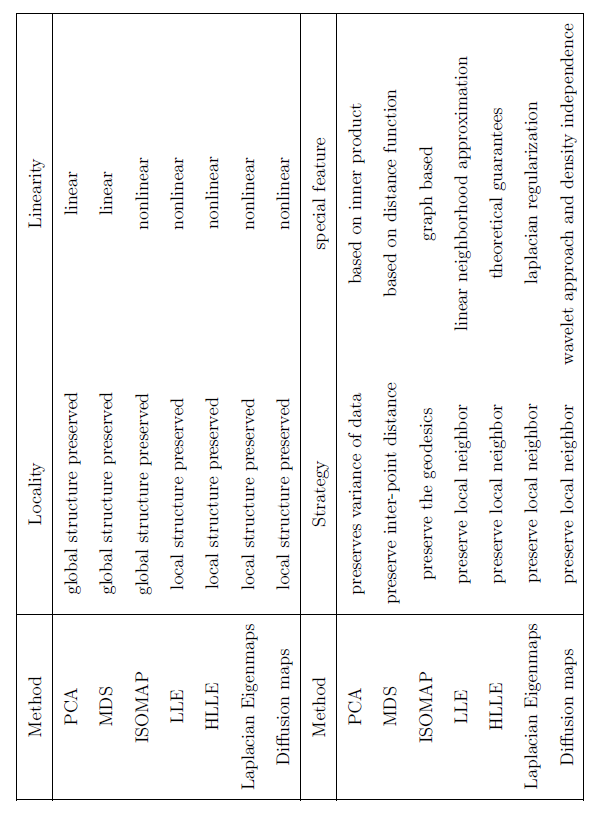
\includegraphics[width=\textwidth]{./Figures/comp_table.png}
\caption {Overview of Manifold Learning Algorithms}
\label{comp} 
\end{center}
\end{figure}

\section{Intrinsic Dimension}
\label{s:id}

Intrinsic Dimension (ID) is defined as the minimal number of parameters necessary to represent the variability of a data set. It is a a key priori
knowledge in computer vision and image processing to improve their performance. Mathematically, a formal definition of the intrinsic dimension is the following, due to \citep{Cama2016}.

\begin{definition}
A data set $\mathbf{X}\subseteq \mathbb{R}^{\mathbf{D}}$ said to have intrinsic dimension equal to $\mathbf{d}$  if its elements lie entirely, without information loss, within a $\mathbf{d}$-dimensional manifold of $\mathbb{R}^{\mathbf{D}}$, where $\mathbf{d} < \mathbf{D}$.
\end{definition}

Most of the existing approach to estimate the intrinsic dimension can be roughly divided into two groups: eigenvalue or projection methods, and geometric methods. Projection or eigenvalues methods, estimate the ID by thresholding the observed eigenspectrum i.e. the spectrum of the eigenvalues output by the global or local PCA. It may be good method for exploratory
data analysis, where one might plot the eigenvalues and look for a clear-cut boundary, but not for providing reliable estimates of intrinsic dimension.

The other, geometric methods exploit the intrinsic geometry of the dataset and are most often based on fractal dimensions or nearest neighbor (NN) distances \citep{Lev2005}.

Finding out the ID of the dimension estimation might become a very complex problem, when data lie on a smooth manifold. In this thesis, we used method proposed by Levina and Bickel \citep{Lev2005} to verify the ID computed by projection and geometric methods. They derive ID by applying the principle of maximum likelihood to the distances between close neighbors. 

%% Chapter 3
\chapter{Manifold Learning} % Main chapter title

\label{Chapter3} % For referencing the chapter elsewhere, use \ref{Chapter1} 

\lhead{Chapter3. \emph{Manifold Learning}} % This is for the header on each page - perhaps a shortened title

%-------------------------------------------------------------------------------
\section*{Overview}
Manifold learning is an emerging and promising approach in nonparametric dimension reduction widely used in image processing, data mining, signals processing and computer vision. The core theme of manifold leaning is to find the most succinct low dimensional structure that is embedded
in a higher dimensional space. Using earlier, the algorithms can work directly in the lower dimensional latent space of the manifold rather high dimensional data space and thus get computationally efficient. In this chapter, we review the representative sample of manifold learning, mathematical developments, as well as some interesting applications. 
%----------------------------------------------------------------------------------------
\section{Introduction}
Most of the datasets encountered in image processing often consist of
a large number of samples each of which are themselves of high dimension.
Further processing of the datum is done either treating it directly or extracting complex features before processing. Nevertheless, it  wither its
entire datum or a set extracted features, the dimensionality of
problems usually remain high. This in turn slows down the processing considerably or sometimes making the treatment even intractable. The task to reducing the computational burden is to reduce the dimensionality of the data. Dimensionality reduction can be thought of as mathematical mapping of high-dimensional data into a meaningful representation of the intrinsic dimensionality. The intrinsic dimensionality of a data set can be defined as the lowest number of variables that can preserve the geometrical structure of the data.


\section{Problem Definition}
Given a set of of high-dimensional training instances $\mathbb{X} = \{x_1, x_2, ...,x_N \}$, where $x_{i} \in \mathbb{R}^D$. We assume that $\mathbb{X}$ approximately lie on a smooth manifold $\mathcal{X}$. The idea of manifold learning algorithms is to find an embedding set $\mathbb{Y} = \{y_1, y_2, ...,y_N \} $ of $\mathbb{X}$ in low dimension space $\mathbb{R}^d$, where $d<D$. The local manifold structure formed by $\mathbb{X}$ in the original space $\mathbb{R}^D$ is preserved in the embedded space $\mathbb{R}^d$.


Manifold Learning can be mainly divided into linear and non linear methods.
Linear methods, which have long been used for analyzing multivariate data, include principal component analysis (PCA) and multidimensional scaling (MDS). A further distinction within non-linear methods is to divide the methods into two classes: one is to preserve the global geometric structure of manifold, such as Isomap \citep{Tene2000} and the other one is to preserve the local neighborhood geometric structure, such as LLE \citep{Roweis2000}.

\section{Linear Methods}
\subsection{Principle Component Analysis}
\label{s:pca}

Principal component analysis (PCA) is a standard algorithm to explain the dispersion of a point cloud by projecting data onto a carefully chosen linear subspace. It reduces the dimensionality of the point cloud while keeping the maximum of variance information. The dispersion in linear subspaces of higher dimension is captured by by building an orthonormal basis such that the projection along each axis has a decreasing maximum variance. 

We consider n points $\mathbf{X} = \{x_1, x_2, ..., x_n\}$ of dimension D from $\mathbb{R}^D$. Also, let us assume $V^{*}$ be a d-dimensional subspace of $\mathbb{R}^D$ and let $ u = \{u_1, u_2, ..., u_D\}$ be an orthonormal basis of $\mathbb{R}^D$ such that $\{u_1, u_2, ..., u_d\}$ is a basis of V. Then each data point is approximated by:

\begin{equation}
y_n = \sum_{i=1}^{d} a_{n,i}u_{i} + \sum_{i=1}^{D+1} a_{n,i}u_{i}
\end{equation}

The below energy function is used to recover $u_1, u_3, ..., u_d$.
\begin{equation}
\mathbb{E} = \frac{1}{N}\sum_{n=1}^{N} \|x_n - y_n\|^{2}
\end{equation}

This is equivalent to minimizing the approximation error. 

\begin{equation}
x_n - y_n = \sum_{i=d+1}^{D} \{(x_n - \bar{x})^T u_i\}u_i
\label{p_3}
\end{equation} 
The above equation \ref{p_3} can be best visualized in the figure \ref{pca}.

\begin{figure}[ht]
\begin{center}
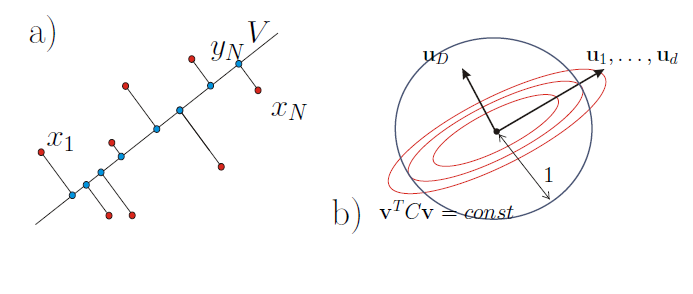
\includegraphics[width=\textwidth]{./Figures/pca.png}
\caption{a) Manifold with original (red) and projected (blue) points. b) Geometry and constraint visualization of optimization function. Pictures taken from Nicolas Thorstensen works \citep{Ety2008}}
\label{pca}
\end{center}
\end{figure}

Now, we can write the energy function as
\begin{equation}
\mathbb{E} = \frac{1}{N}\sum_{n=1}^{N}\sum_{i=d+1}^{D} (x_n^{T}u_{i}- \bar{x}^{T}u_i)^2 = \sum_{i=d+1}^{D}u_{i}^{T}\mathbf{C}u_{i}
\end{equation}

$\mathbf{C}$ is defined as covariance matrix, $\mathbf{C} = \frac{1}{N}\sum_{n=1}^{N}(x_n-\bar{x})(x_n -\bar{x})^2$. Our optimization problem look like
\begin{equation}
\begin{aligned}
& \underset{D}{\text{minimize}}
&& \mathbb{E} = u_{D}^{T}\mathbf{C}u_{D} \\
& \text{subject to}
&& u_{D}^{T}u_{D} = 1
\end{aligned}
\end{equation}
Now using Lagrange multipliers, we solve this constraint optimization problem as
\begin{equation}
u_{D}^{T}\mathbf{C}u_{D}+\lambda(1-u_{D}^{T}u_{D})=0
\label{LM}
\end{equation}

The solution off the above equation gives standard form eigenvalue problem $\mathbf{C}u_D =\lambda u_D$. The geometry of the minimization problem is illustrated in figure \ref{pca} b).

We take an input image \ref{app_pca} (A), which is sequence of vector in $\mathbb{R}^{4096}$ representing the brightness values of $64\times64$ pixel image of the face. The 1st dimension representing embedding correlates with intrinsic-dimension of one, which is left-right pose. The two-dimensional projection of original input image found by PCA is shown in figure \ref{app_pca} (B).

\begin{figure}
\centering
\begin{subfigure}{.5\textwidth}
  \centering
  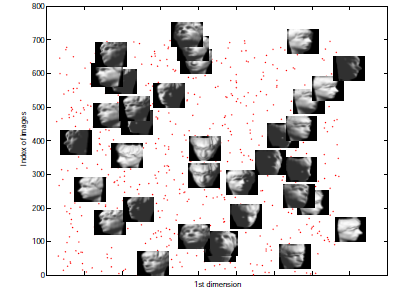
\includegraphics[width=\linewidth]{./Figures/original.png}
\caption{Input}
%  \label{fig:sub1}
\end{subfigure}%
\begin{subfigure}{.5\textwidth}
  \centering
  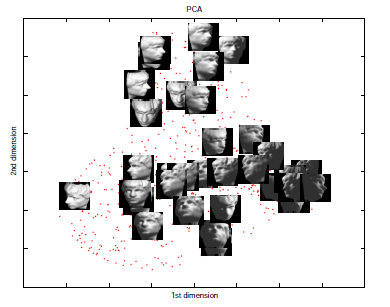
\includegraphics[width=\linewidth]{./Figures/o_pca.png}
  \caption{Output}
%  \label{fig:sub2}
\end{subfigure}
\caption{Application of PCA. }
\label{app_pca}
\end{figure}

\subsection{Multi-Dimensional Scaling}
\label{s:MDS}

The Multi-Dimensional Scaling (MDS), is a PCA-like technique that maps the original high dimensional space to a lower dimensional space by preserving pairwise distances. Figure \ref{app_mds} shows an example of MDS, where pairwise distance is preserved. MDS \citep{Cox2000} is applied when it difficult to calculate   covariance matrix from the dataset, when data are, for instance, qualitative or infinite dimensional, when only a point-wise distance is known or also when the size $\mathbb{D}$ of the sample set is lower than the dimension of data \citep{Ety2008}.


MDS addresses the problem of finding d-dimensional Euclidean coordinates
for each data sample ($x_i \in \mathbf{X}$) so that the pairwise distance ($d$) of their Euclidean coordinates match the original pairwise distance as closely as possible. 

We define $N \times N$ euclidean distance or affinity matrices $\mathbf{D}$ as symmetric, $d_{ii}=0$ and $d_{ij}>0$, if $i \neq j$. With $\mathbf{D}$ matrix in hand, the MDS algorithm attempts to find $N$ data points $\mathbf{Y} = y_1, y_2, y_3,...,y_N$ in $\mathbb{R}^d$ such that distance matrix is preserved as depicted in the figure \ref{mds}.


\begin{figure}
\centering
\begin{subfigure}{.5\textwidth}
  \centering
  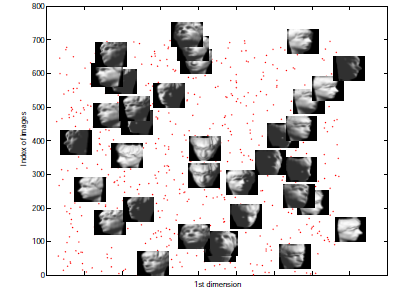
\includegraphics[width=\linewidth]{./Figures/original.png}
\caption{Input}
%  \label{fig:sub1}
\end{subfigure}%
\begin{subfigure}{.5\textwidth}
  \centering
  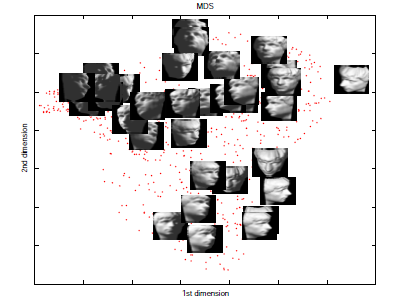
\includegraphics[width=\linewidth]{./Figures/o_mds.png}
  \caption{Output}
%  \label{fig:sub2}
\end{subfigure}
\caption{Application of MDS.}
\label{app_mds}
\end{figure}

\begin{figure}[ht]
\begin{center}
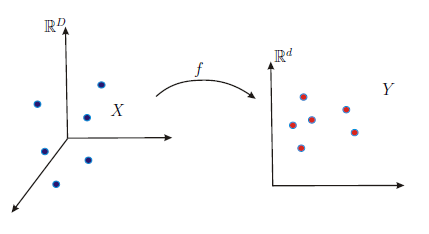
\includegraphics[width=\textwidth]{./Figures/mds.png}
\caption {Multi-Dimensional Scaling}
\label{mds}
\end{center}
\end{figure}

In particular, we try to optimize following function:

\begin{equation}
\begin{aligned}
& \underset{\mathbf{Y}}{\text{Min}}
&& \sum_{i=1}^{N}\sum_{i=1}^{N}(d_{ij}^{\mathbf{X}}-d_{ij}^{\mathbf{Y}})^{2}
\label{mds:1}
\end{aligned}
\end{equation}

where, $d_{ij}^{\mathbf{X}}$ and $d_{ij}^{\mathbf{Y}}$ is normed distance from sample point $x_{i}$ and $x_{i}$ respectively. Converting distance $\mathbf{D}^{\mathbb{X}}$ matrix into kernel matrix of inner product yields:

\begin{equation}
\mathbf{X}^{T}\mathbf{X} = -\frac{1}{2}\mathbf{J}\mathbf{D}^{\mathbb{X}}
\end{equation}
where $\mathbf{J} = \mathcal{I}d_{N}-\frac{1}{N}\mathbf{1}\mathbf{1}^{T}$. Now the equation \ref{mds:1} can be reduced into

\begin{equation}
\begin{aligned}
& \underset{\mathbf{Y}}{\text{Min}}
&& \sum_{i=1}^{N}\sum_{i=1}^{N}(x_{i}^{T}x_{j}-y_{i}^{T}y_{j})^{2}
\label{mds:2}
\end{aligned}
\end{equation}


Solving equation \ref{mds:2} as shown in Cox and Cox paper\citep{Cox2000} gives $\mathbf{Y}=\lambda^{\frac{1}{2}}\mathbf{U}^{T}$. Here, $\mathbf{U}$ is eigenvector of $\mathbf{X}^{T}\mathbf{X}$ corresponding to top d eigenvalues, and $\lambda$ is top d eigenvalues of $\mathbf{X}^{T}\mathbf{X}$.


MDS can be generalized into to geodesic distances between point samples from
a non-linear manifold. But a non-convex energy function coming out makes it  
tedious to optimize. In the next section we will provide an overview of non-linear manifold algorithms.


\section{Non-Linear Methods}

Linear methods such as PCA and MDS fails to produce desired results when the data is sampled from non linear manifolds \citep{Thor2009}. We now review representative non-linear methods in manifold learning in this section with assumption that the data is distributed along a d-dimensional submanifold $\mathcal{X}$ embedded in $\mathbb{R}^{D}$.

\subsection{Graph-based Algorithms}

Manifold learning based on graph based algorithms often relies on preserving the geometric structure in the neighborhood of some points. The important step is to construct a graph using $K$-nearest neighbor graph or $\epsilon$-neighborhood and apply MDS as previously detailed.

\subsubsection{Isomap}
\label{s:isomap}

Isomap was proposed by Joshua Tenenbaum, Vin de Silva and John Langford in Science \citep{Tene2000}. It is an extended version of MDS for data lying on smooth non-linear manifold. Unlike MDS, the pairwise distance matrix in Isomap is replaced by the matrix of pairwise geodesic distances approximated by distances in graphs. The algorithm proceeds in three steps. First a distance $d(x; y)$ is considered in the data space. Then, a neighborhood graph based on a $\epsilon$-neighborhood or $k$-nearest neighbor points is build with following weights $D_{ij} = d(xi; xj)$ if an edge link
exists between points $x_i$ and $x_j$ , otherwise $D_{ij} = 1$. The pairwise distance matrix $\mathbf{D}$ is then calculated using a Dijkstra-like algorithm in the graph. Finally, the data via MDS is embedded so as to preserve these distances. A two-dimensional projection using isomap is shown in the figure \ref{app_iso} with k=6.

\begin{figure}
\centering
\begin{subfigure}{.5\textwidth}
  \centering
  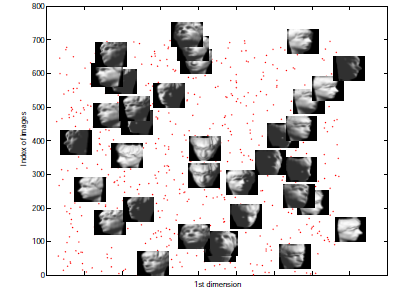
\includegraphics[width=\linewidth]{./Figures/original.png}
\caption{Input}
%  \label{fig:sub1}
\end{subfigure}%
\begin{subfigure}{.5\textwidth}
  \centering
  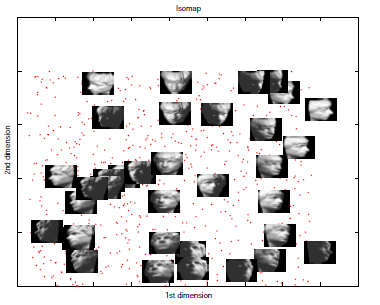
\includegraphics[width=\linewidth]{./Figures/o_iso.png}
  \caption{Output}
%  \label{fig:sub2}
\end{subfigure}
\caption{Application of Isomap}
\label{app_iso}
\end{figure}

Precautionary measure should be taken while calculating distances between far apart points on the manifold, which can be very close in the data space as discussed in the figure \ref{isomap}.
\begin{figure}[ht]
\begin{center}
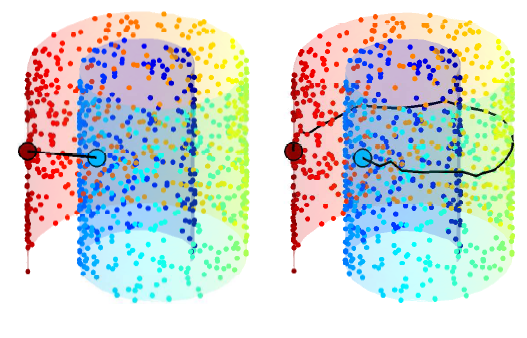
\includegraphics[width=\textwidth]{./Figures/isomap.png}
\caption {Multi-Dimensional Scaling. Left: Distance between two
points using a distance in the data space. Right: Distance between two points
using an approximated geodesic path. Image taken from Patrick Etyngier work \citep{Ety2008}.}
\label{isomap}
\end{center}
\end{figure}

\subsubsection{Locally linear Embedding}
\label{s:lle}
Locally linear Embedding (LLE) is a manifold mapping dimension reduction algorithm introduced by Roweis \& Saul \citep{Roweis2000}. It aims at recovering the low dimensional geometry of the data by looking at the local interaction between data points. The construction of a nearest neighbor graph recovers the local interactions. Then further processing is done to reduce the dimensionality of the data and provide a parametrization in a d- dimensional hyperplane. LLE algorithm can be summarized in the following steps:

\begin{enumerate}
\item  Neighborhood graph $\mathcal{G}$ is build on the dataset $\mathbb{X}$ using K-nearest neighbour method. 
\item Weights $W_{ij}$ are calculated to each of the nearest neighbours pair $(x_i, y_i)$ by minimising the cost function:
      \begin{equation}
     \epsilon(W) = \sum_{i}\vert x_{i} - \sum_{j=1}^k W_{ij} x_{j}\vert^{2}
    \end{equation}
   
\item The inner products between each point $x_i$ and each of its nearest neighbours are computed to produce gram positive-semidefinite matrix, $G_{jk} = (x -x_j)^T(x-x_i)$.
\item  The reconstruction weights are then computed using:
    \begin{equation}
     W_{ij} = \sum_{k}\mathbb{G}-{jk}^{-1}(G_{jk}+\lambda)
    \end{equation}
    such that, $W_{ij} =0 $ if $x_{j}$ is not one of the nearest neighbours of $x_{i}$ and $\sum_{j} W_{ij} = 1$)
    
\item Finally the embedded $\mathbb{Y}$ which will make up the final output data are calculated by minimising a second cost function:
    \begin{equation}
     \Phi(Y) = \sum_{i}\vert y_{i}-\sum_{j}W_{ij}y_{j}\vert^{2}
    \end{equation}
We also constraint $\sum_{i}y_{i} = 0$ to centre the projection on the origin. The other constraint is imposed in order to avoid degenerate solutions;
    \begin{equation}
     \frac{1}{n}\sum_{i}y_{i}y_{i}^{T} = I
    \end{equation}
    where I is the d$\times$d identity matrix.
    
\item     This cost function now defines a quadratic form containing the N$\times$N symmetric matrix $M_{ij}$:
    \begin{equation}
     \Phi(I) =\sum_{ij}M_{ij}y_{i}y_{i}^{T}
    \end{equation}
    where $M_{ij} = \delta_{ij}-W_{ij}-W_{ij}+\sum_{k}W_{ki}W_{kj}$ and $\delta_{ij} = 1$ if $i = j$ and $\delta_{ij} = 0$ otherwise.
\item The embedding $\mathbb{Y}$ is then given by the the lowest d+1 eigenvectors of the matrix $M_{ij}$. The bottom eigenvector representing a 
free translation mode of eigenvalue 0 is left out in order to find the optimum embedding.

\end{enumerate}

The geometry the optimization problem is depicted in figure \ref{lle}.

\begin{figure}[ht]
\begin{center}
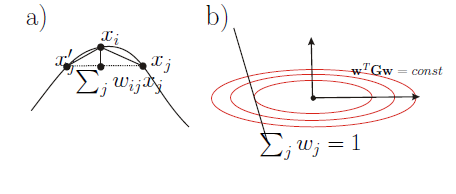
\includegraphics[width=\textwidth]{./Figures/lle.png}
\caption {LLE. a) $x_i$ is appropriated by its neighborhood $(x_{j}^{'}, x_{j})$. b) The black line touching the level set at a single point defines the constraints}
\label{lle} 
\end{center}
\end{figure}

A two-dimensional projection of the original input by using with k=5 is shown in the figure \ref{app_lle}.
\begin{figure}
\centering
\begin{subfigure}{.5\textwidth}
  \centering
  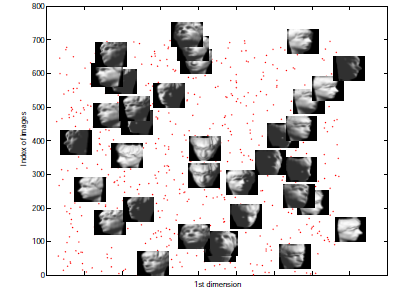
\includegraphics[width=\linewidth]{./Figures/original.png}
\caption{Input}
%  \label{fig:sub1}
\end{subfigure}%
\begin{subfigure}{.5\textwidth}
  \centering
  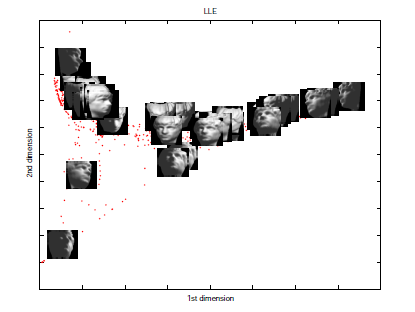
\includegraphics[width=\linewidth]{./Figures/o_lle.png}
  \caption{Output}
%  \label{fig:sub2}
\end{subfigure}
\caption{Application of LLE}
\label{app_lle}
\end{figure}

\subsection{Laplacian-based Algorithms}
Laplacian based algorithms assume that data have a structure of low dimensional manifold embedded in a higher dimensional space. The maps are constructed into a low dimensional space preserving the local neighborhood topology. In this part, we give outlines of representative laplacian based algorithms.

\subsubsection{Laplacian Eigenmaps}
\label{s:le}
Laplacian Eigenmaps were introduced by Belkin \citep{Bel2002}. Its intent is
to embed the observed data $\mathbf{X}$ into $\mathbb{R}^d$ by first constructing the $k$-nearest-neighbor or $\epsilon$-graph $\mathcal{G}$ from $\mathbf{X}$. In the $k$-nearest-neighbor graph, an edge is present between $x_i$ and $x_j$ if $x_i$ is among the $k$ nearest neighbors of $x_j$ or vice versa. In the $\epsilon$-graph, $x_i$ and $x_j$ are adjacent if $\|x_i-x_j\|^2<\epsilon$ for a given threshold parameter $\epsilon$. The weighted adjacency matrix of $\mathcal{G}$ is defined as $\mathbf{W}$, $$\mathbf{W}_{ij}=\begin{cases} \mathbf{K}_{ij} &\mbox{ if } \{i,j\}\in E\\
                0 &\mbox{ else}, \end{cases}$$ and let $\mathbf{D}\in\mathbb{R}^{N\times N}$ be the diagonal matrix defined by $\mathbf{D}_{ii}=\sum_{j}\mathbf{W}_{ij}$ for $i\in[N]$.
                
Then the normalized weighted graph Laplacian of $\mathbf{G}$ \citep{Bel2002}
is given by $\mathbf{W}=\mathbf{D}^{-1/2}\mathbf{W}\mathbf{D}^{-1/2}$.
If we represent eigendecomposition of $\mathbf{W}$  by $\mathbf{W}=\mathbf{U}\Lambda \mathbf{U}^\top$ with the diagonal entries of $\Lambda$ non-increasing, then Laplacian eigenmaps embeds $\mathbf{X}$ via
$\mathbf{U}[:,2:d+1]$---the first $d$ nontrivial eigenvectors of $\mathbf{W}$. The local geometry of $\mathbf{X}$ is optimally preserved in a least squares sense by the former.
 
A two-dimensional projection of the original input by using with k=9 is shown in the figure \ref{app_le}.
 
\begin{figure}
\centering
\begin{subfigure}{.5\textwidth}
  \centering
  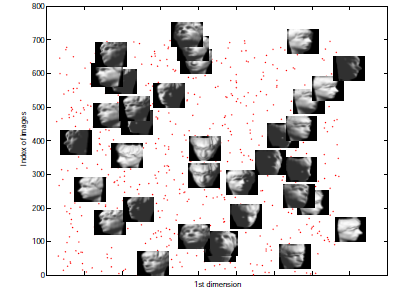
\includegraphics[width=\linewidth]{./Figures/original.png}
\caption{Input}
%  \label{fig:sub1}
\end{subfigure}%
\begin{subfigure}{.5\textwidth}
  \centering
  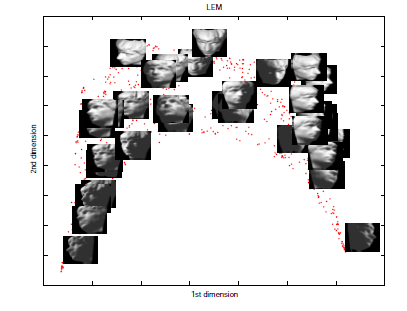
\includegraphics[width=\linewidth]{./Figures/o_le.png}
  \caption{Output}
%  \label{fig:sub2}
\end{subfigure}
\caption{Application of Laplacian Eigenmaps}
\label{app_le}
\end{figure}



\subsubsection{Diffusion Maps}
\label{s:dm}

The objective of Diffusion Maps (DM) is to define a metric, named the diffusion distance, that measures the connectivity between points in an arbitrary set. We will follow the construction of DM as described
in the paper by Lindenbaum and others \citep{Lind2015}.

Representing the high dimensional input dataset \begin{math} \mymat{X} \end{math}, the DM framework contains the following steps:

\begin{enumerate}

\item A kernel function  \begin{math}{{\cal{K}} : \mymat{X}\times{\mymat{X}}\longrightarrow{\mathbb{R}}  }
	\end{math} is chosen to define an anisotropic transition matrix, represented by $\mymat{K} \in {\mathbb{R}^{D \times D}}$. It satisfies the following properties for all 
	\begin{math}{(\myvec{x}_i,\myvec{x}_j) \in {\mymat{X}} }
	\end{math}.
	
	\begin{enumerate}
	
     \item Symmetry: \begin{math}{K_{i,j}={\cal{K}}(\myvec{x}_i,\myvec{x}_j)={\cal{K}}(\myvec{x}_j,\myvec{x}_i) }
	\end{math}, 
	
	\item Positive semi-definiteness: \begin{math}{ \myvec{v}_i^T  \mymat{K}  \myvec{v}_i \geq 0 }\end{math} for all $\myvec{v}_i \in
	\mathbb{R}^D$ and 
	
	\item Non-Negativity \begin{math}{{\cal{K}}(\myvec{x}_i,\myvec{x}_j)
		\geq 0. }
	\end{math}
	\end{enumerate}
	
\item {When we normalize the kernel using  $\mymat{M}$; where  \begin{math} M_{i,i}=\underset{j}{\sum}{K_{i,j}} \end{math}, the following matrix elements are computed:  
\begin{equation}
		{P_{i,j}^x={\cal{P}}(\myvec{x}_i,\myvec{x}_j)=[{{\mymat{M}}^{-1}{\mymat{K}}  }}]_{i,j}
		\label{EquationPDM}
		.\end{equation}
		
		 The resulting matrix $ \mymat{P}^x \in \mathbb{R}^{D
			\times D} $ is actually transition kernel of a 
		Markov chain on $\mymat{X}$ such that the expression
		${[{(\mymat{P}^x)^t}]_{i,j}}=p_t(\myvec{x}_i$,$\myvec{x}_j)$
		describes the transition probability from point
		\begin{math}{\myvec{x}_i}
		\end{math} to point \begin{math}{\myvec{x}_j}
		\end{math} in $t$ steps.
	}
\item{ Next, the spectral decomposition is applied to matrix \begin{math}  \mymat{P}^x \end{math} to obtain a sequence of eigenvalues  \begin{math}{\lbrace {\lambda_d}\rbrace }
		\end{math} and normalized eigenvectors \begin{math}{\lbrace{{\mbox{\boldmath${\psi}$}}_d}\rbrace }
		\end{math} that satisfies ${ {\mymat{P}^x}  {\mbox{\boldmath${\psi}$}_d} =\lambda_m{\mbox{\boldmath${\psi}$}}_d, d=0,...,D-1}
		$; }
\item{
		Defining a new representation for the dataset $\mymat{X}$
		\begin{equation}{ \myvec{\Psi}_t{(\myvec{x}_i)}:   \myvec{x}_i
			\longmapsto \begin{bmatrix} { \lambda_1^{t}\psi_1[i]} , {
				\lambda_2^{t}\psi_2[i]} , { \lambda_3^{t}\psi_3[i]} , {.} {.} {.}
			,
			
			{\lambda_{D-1}^{t}\psi_{D-1}[i]}\\
			
			\end{bmatrix}^T \in{\mathbb{R}^{D-1}} },
		\end{equation}
		where $t$ is the selected number of steps and $\psi_d[i]$ denotes the $i^{\rm{th}}$ element of ${\mbox{\boldmath${\psi}$}_d}$.
		
Now the Euclidian distance between two data points is equal to the weighted $L_2$ distance between the conditional probabilities ${{p}_t(\myvec{x}_i,:)}$, and ${{p}_t(\myvec{x}_j,:)}$, $i,j=1,...,D$ (the $i$-th and $j$-th rows of $\myvec{P}^t$), which is referred as the Diffusion Distance
			\begin{equation}{ \label{EqDist} { {\cal{D}}^2_t( \myvec{x}_i,\myvec{x}_j)=||{\mymat{\Psi}_t{(\myvec{x}_i)}}-{\mymat{\Psi}_t{(\myvec{x}_j)}}||^2={  \sum_{d\geq{1}} {\lambda}^{2t}_d (\psi_d[i]-\psi_d[j])^2 }}=\\
			||{p_t}(\myvec{x}_i,:)-{p_t}(\myvec{x}_j,:)||^2_{\tiny\mymat{W}^{-1}}},
			\end{equation}
			where $\mymat{W}$ is a diagonal matrix with elements
			$W_{i,i}=\frac{D_{i,i}}{\sum_{i=1}^M D_{i,i}}$.}
	\item{The desired accuracy $\delta \geq 0$ is chosen for the diffusion distance defined by Eq. (\ref{EqDist}) such that
		$s(\delta,t)=\text{max} \{\ell\in \mathbb{N}$  such that   $|\lambda_{\ell}|^t > \delta |\lambda_1|^t \}  $. By using $\delta$, a new mapping
		of $s(\delta,t)$ dimensions is defined as \\ \begin{math} {\Psi^{(\delta)}_t :  X \rightarrow \begin{bmatrix}
			{ \lambda_1^{t}\psi_1[i]} , { \lambda_2^{t}\psi_2(i)} , {
				\lambda_3^{t}\psi_3[i]} , {.} {.} {.}   ,
			
			{\lambda_{s}^{t}\psi_{s}[i]}\\
			
			\end{bmatrix}^T \in \mathbb{R}^{s(\delta,t)}} \end{math} .  }
\end{enumerate}

As discussed above, diffusion distance reflects the intrinsic geometry of the data set defined via the adjacency graph in a diffusion process.

\section{Other manifold learning algorithms}

Many other Laplacian based techniques exist in literature to reduce the dimensionality of a point cloud which were not dicussed in this chapter. For example, Maximum Variance Unfolding (MVU)\citep{Ety2008}, which links most of Laplacian-based methods such as LE, LLE and Isomap. Another important approach which is derived from the LLE framework is called Hessian eigenmaps\citep{Ety2008}. The methods is widely used when the underlying embedding is not convex. In figure \ref{comp} taken from Thorstensen work \citep{Thor2009} lists the general properties for manifold learning algorithms.

\begin{figure}[ht]
\begin{center}
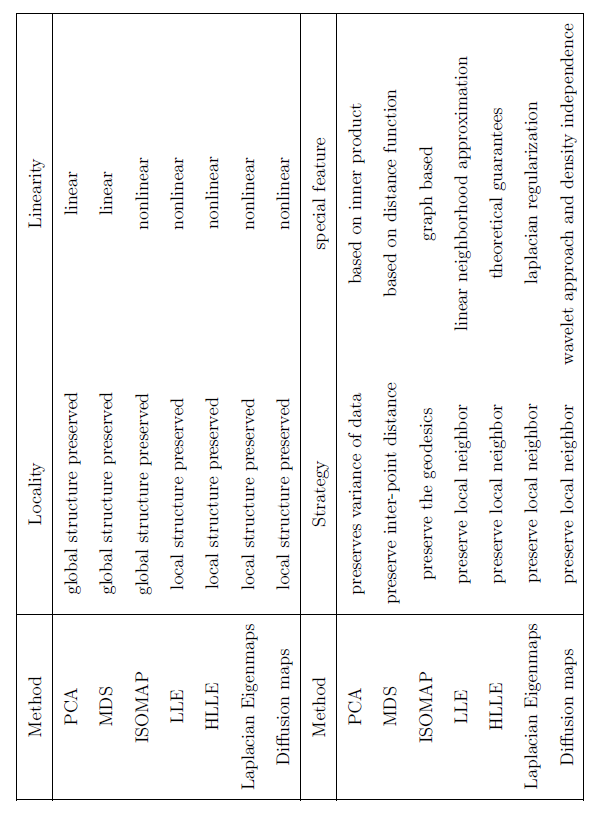
\includegraphics[width=\textwidth]{./Figures/comp_table.png}
\caption {Overview of Manifold Learning Algorithms}
\label{comp} 
\end{center}
\end{figure}

\section{Intrinsic Dimension}
\label{s:id}

Intrinsic Dimension (ID) is defined as the minimal number of parameters necessary to represent the variability of a data set. It is a a key priori
knowledge in computer vision and image processing to improve their performance. Mathematically, a formal definition of the intrinsic dimension is the following, due to \citep{Cama2016}.

\begin{definition}
A data set $\mathbf{X}\subseteq \mathbb{R}^{\mathbf{D}}$ said to have intrinsic dimension equal to $\mathbf{d}$  if its elements lie entirely, without information loss, within a $\mathbf{d}$-dimensional manifold of $\mathbb{R}^{\mathbf{D}}$, where $\mathbf{d} < \mathbf{D}$.
\end{definition}

Most of the existing approach to estimate the intrinsic dimension can be roughly divided into two groups: eigenvalue or projection methods, and geometric methods. Projection or eigenvalues methods, estimate the ID by thresholding the observed eigenspectrum i.e. the spectrum of the eigenvalues output by the global or local PCA. It may be good method for exploratory
data analysis, where one might plot the eigenvalues and look for a clear-cut boundary, but not for providing reliable estimates of intrinsic dimension.

The other, geometric methods exploit the intrinsic geometry of the dataset and are most often based on fractal dimensions or nearest neighbor (NN) distances \citep{Lev2005}.

Finding out the ID of the dimension estimation might become a very complex problem, when data lie on a smooth manifold. In this thesis, we used method proposed by Levina and Bickel \citep{Lev2005} to verify the ID computed by projection and geometric methods. They derive ID by applying the principle of maximum likelihood to the distances between close neighbors. 
 
%----------------------------------------------------------------------------------------
%	THESIS CONTENT - CHAPTER3
%----------------------------------------------------------------------------------------

%\mainmatter % Begin numeric (1,2,3...) page numbering

\pagestyle{fancy} % Return the page headers back to the "fancy" style

% Include the chapters of the thesis as separate files from the Chapters folder
% Uncomment the lines as you write the chapters

% Chapter 4
\chapter{Dimension Reduction and Image Process} % Main chapter title

\label{Chapter4} % Fr referencing the chapter elsewhere, use \ref{Chapter1} 

\lhead{Chapter 4. \emph{Dimension Reduction and Image Process}} % This is for the header on each page - perhaps a shortened title

%----------------------------------------------------------------------------------------



%----------------------------------------------------------------------------------------

%% Chapter 4
\chapter{Dimension Reduction and Image Process} % Main chapter title

\label{Chapter4} % Fr referencing the chapter elsewhere, use \ref{Chapter1} 

\lhead{Chapter 4. \emph{Dimension Reduction and Image Process}} % This is for the header on each page - perhaps a shortened title

%----------------------------------------------------------------------------------------



%----------------------------------------------------------------------------------------
 
%----------------------------------------------------------------------------------------
%	THESIS CONTENT - CHAPTER4
%----------------------------------------------------------------------------------------

%\mainmatter % Begin numeric (1,2,3...) page numbering

\pagestyle{fancy} % Return the page headers back to the "fancy" style

% Include the chapters of the thesis as separate files from the Chapters folder
% Uncomment the lines as you write the chapters

% Chapter 5
\chapter{Anomaly Detection} % Main chapter title

\label{Chapter5} % Fr referencing the chapter elsewhere, use \ref{Chapter1} 

\lhead{Chapter 5. \emph{Anomaly Detection}} % This is for the header on each page - perhaps a shortened title

%----------------------------------------------------------------------------------------


%----------------------------------------------------------------------------------------

%% Chapter 5
\chapter{Anomaly Detection} % Main chapter title

\label{Chapter5} % Fr referencing the chapter elsewhere, use \ref{Chapter1} 

\lhead{Chapter 5. \emph{Anomaly Detection}} % This is for the header on each page - perhaps a shortened title

%----------------------------------------------------------------------------------------


%----------------------------------------------------------------------------------------
 
%----------------------------------------------------------------------------------------
%	THESIS CONTENT - CHAPTER5
%----------------------------------------------------------------------------------------

%\mainmatter % Begin numeric (1,2,3...) page numbering

\pagestyle{fancy} % Return the page headers back to the "fancy" style

% Include the chapters of the thesis as separate files from the Chapters folder
% Uncomment the lines as you write the chapters

% Chapter 6
\chapter{Conclusion} % Main chapter title

\label{Chapter6} % Fr referencing the chapter elsewhere, use \ref{Chapter1} 

\lhead{Chapter 6. \emph{Conclusion}} % This is for the header on each page - perhaps a shortened title

%----------------------------------------------------------------------------------------

\section{Conclusions}
\begin{enumerate}

\item The enormous blockchain (60 GB as of now) and the newer bitcoin clients indexing the full blockchain using LevelDB had made earlier public available software obsolete. The thesis develops an open source blockchain parsing tools to extract agent resolved data, which can be used to extend the stucked research in bitcoin transaction dynamics.

\item The validation of the data parsed from our tool is then checked by
reproducing the ”Mathew Effect” phenomenon from prominent paper using their original matlab code, but with our own data. The transaction dynamics in the bitcoin as money flow on the transaction network, support popular hypothesis in economics having roots in preferential attachment, called Matthew effect or the "rich get richer phenomenon".

\item By using the agent resolved data, the case study of silk road arrest is illustrated with the transaction graph with details. It paves the way to understand the important events in bitcoin based on transaction.

\item By defining quantitative measure of transformation over time, in terms of similarity index using different kernels, we infer that there is correspondence between network structure and exchange price in bitcoin. It also concludes that choice of graph kernels as per the graph structure plays important role on problem related to graph isomorphism. 

\item We extend deep graph kernels \citep{Yanardag2015},
involving propagation kernels, unseen in literature, to solve graph isomorphism problem, which gives extremely agreeable results.

\item By defining quantitative measure of transformation over time, in terms of similarity index using different kernels, we infer that there is correspondence between network structure and exchange price in bitcoin, which is first step in price forecasting.

\end{enumerate}

\section{Future Work}

\begin{enumerate}

\item On transactions data front, the future work would be to transform the data set into a simplified one indexed by user entity rather than
address to do some other meaningful studies, like identifying cluster, market player and linking events to predict bubbles.

\item  The possible extension of our work would be to leverage on blockchain network features, as a basis to conduct deep learning learning
prediction on the price change of Bitcoin.

\end{enumerate}
%----------------------------------------------------------------------------------------

%% Chapter 6
\chapter{Conclusion} % Main chapter title

\label{Chapter6} % Fr referencing the chapter elsewhere, use \ref{Chapter1} 

\lhead{Chapter 6. \emph{Conclusion}} % This is for the header on each page - perhaps a shortened title

%----------------------------------------------------------------------------------------

\section{Conclusions}
\begin{enumerate}

\item The enormous blockchain (60 GB as of now) and the newer bitcoin clients indexing the full blockchain using LevelDB had made earlier public available software obsolete. The thesis develops an open source blockchain parsing tools to extract agent resolved data, which can be used to extend the stucked research in bitcoin transaction dynamics.

\item The validation of the data parsed from our tool is then checked by
reproducing the ”Mathew Effect” phenomenon from prominent paper using their original matlab code, but with our own data. The transaction dynamics in the bitcoin as money flow on the transaction network, support popular hypothesis in economics having roots in preferential attachment, called Matthew effect or the "rich get richer phenomenon".

\item By using the agent resolved data, the case study of silk road arrest is illustrated with the transaction graph with details. It paves the way to understand the important events in bitcoin based on transaction.

\item By defining quantitative measure of transformation over time, in terms of similarity index using different kernels, we infer that there is correspondence between network structure and exchange price in bitcoin. It also concludes that choice of graph kernels as per the graph structure plays important role on problem related to graph isomorphism. 

\item We extend deep graph kernels \citep{Yanardag2015},
involving propagation kernels, unseen in literature, to solve graph isomorphism problem, which gives extremely agreeable results.

\item By defining quantitative measure of transformation over time, in terms of similarity index using different kernels, we infer that there is correspondence between network structure and exchange price in bitcoin, which is first step in price forecasting.

\end{enumerate}

\section{Future Work}

\begin{enumerate}

\item On transactions data front, the future work would be to transform the data set into a simplified one indexed by user entity rather than
address to do some other meaningful studies, like identifying cluster, market player and linking events to predict bubbles.

\item  The possible extension of our work would be to leverage on blockchain network features, as a basis to conduct deep learning learning
prediction on the price change of Bitcoin.

\end{enumerate}
%----------------------------------------------------------------------------------------
 
%----------------------------------------------------------------------------------------
%	THESIS CONTENT - CHAPTER6
%----------------------------------------------------------------------------------------

%\mainmatter % Begin numeric (1,2,3...) page numbering

\pagestyle{fancy} % Return the page headers back to the "fancy" style

% Include the chapters of the thesis as separate files from the Chapters folder
% Uncomment the lines as you write the chapters

%----------------------------------------------------------------------------------------
%	THESIS CONTENT - APPENDICES
%----------------------------------------------------------------------------------------

\addtocontents{toc}{\vspace{2em}} % Add a gap in the Contents, for aesthetics

\appendix % Cue to tell LaTeX that the following 'chapters' are Appendices

% Include the appendices of the thesis as separate files from the Appendices folder
% Uncomment the lines as you write the Appendices

% Appendix A
\chapter{Manifold learning algorithms for artificial data} % Main appendix title
\label{AppendixA} % For referencing this appendix elsewhere, use \ref{AppendixA}

\lhead{Appendix. \emph{Manifold learning algorithms for artificial data}} % This is for the header on each page - perhaps a shortened title

\begin{figure}[ht]
\begin{center}
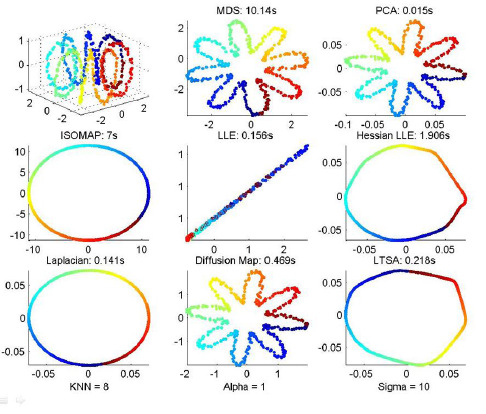
\includegraphics[width=\textwidth]{./Figures/App1.png}
\caption{ Manifold learning algorithms comparison using Swiss Roll. MDS and PCA fails to unroll Swiss Roll; LLE and Laplacian fails to perform too; Diffusion maps couldn't unroll Swiss Roll. }
%\label{pca}
\end{center}
\end{figure}


\begin{figure}[ht]
\begin{center}
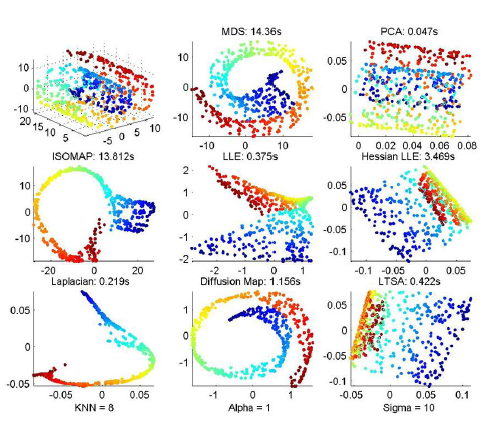
\includegraphics[width=\textwidth]{./Figures/App2.png}
\caption{ Manifold learning algorithms comparison using Toroidal Helix. ISOMAP, LLE, Laplacian, and Diffusion Map unraveled Toroidal Helix into a
circle, which is correct. PCA and MDS fails to perform. }
%\label{pca}
\end{center}
\end{figure}
%\input{Appendices/AppendixB}
%\input{Appendices/AppendixC}

\addtocontents{toc}{\vspace{2em}} % Add a gap in the Contents, for aesthetics
%\addcontentsline{toc}{chapter}{Bibliography}
\backmatter


%----------------------------------------------------------------------------------------
%	BIBLIOGRAPHY

%----------------------------------------------------------------------------------------
\clearpage % Start a new page
\begin{thebibliography}{99}
\setlength{\parskip}{1em}

\bibitem{Thor2009} Thorstensen, Nicolas. 
\newblock Manifold learning and applications to shape and image processing.
\newblock {\em PhD Thesis, Ecole des Ponts ParisTech}.
\newblock \url {https://pastel.archives-ouvertes.fr/pastel-00005860/file/Thesis.pdf}, 2009.


\bibitem{Tal2008} Talwalkar, A and Kumar, S and Rowley, H. 
\newblock Large-scale manifold learning.
\newblock {\em 2008 IEEE Conference on Computer Vision and Pattern Recognition}. 1-8, June, 2008.


\bibitem{Ety2008} Etyngier, Patrick . 
\newblock Statistical learning, Shape Manifolds and Applications to Image Segmentation.
\newblock {\em PhD thesis, Ecole Nationale des Ponts et Chausees}.
\newblock \url {http://imagine.enpc.fr/publications/papers/PhD08.pdf}, 9, 41, 135, 2008.

\bibitem{Bel2002} Belkin, Mikhail and Partha Niyogi. 
\newblock Laplacian Eigenmaps and Spectral Techniques for Embedding and Clustering.
\newblock {\em Advances in Neural Information Processing Systems 14}.
\newblock \url {http://papers.nips.cc/paper} MIT Press, 585--591, 2002.

\bibitem{Boot2003} Boothby, W.M.
\newblock: An Introduction to Differential Manifolds and Riemannian Geometry. 
\newblock {\em . Academic Press}, London, 2003.


\bibitem{Tene2000} Tenenbaum, J,  De Silva, V and Langford, J. 
\newblock A global geometric framework for nonlinear dimension reduction.
\newblock {\em Science}, vol. 290, 2000.

\bibitem{Roweis2000} Roweis ST and Saul LK.
\newblock  Nonlinear dimensionality reduction by locally linear embedding.
\newblock {\em Science}, 290:2323–2326, 2000.

\bibitem{Cox2000} Cox, Trevor and Cox, Michael.
\newblock Multidimensional Scaling.
\newblock {\em  Second Edition. Chapman \& Hall/CRC}, September 2000.

\bibitem{Lind2015} Lindenbaum, Ofir and Yeredor, Arie and Salhov, Moshe and Averbuch, Amir.
\newblock MultiView Diffusion Maps.
\newblock {\em CoRR}.
\newblock \url {https://arxiv.org/pdf/1508.05550.pdf}, 2015.

\bibitem{Cama2016} Camastra, Francesco and Staiano, Antonino.
\newblock  Intrinsic dimension estimation: Advances and open problems.
\newblock {\em Inf. Sci.},328,C, 26-41, 2016.

\bibitem{Lev2005} Levina, Elizaveta  and Bickel, Peter.
\newblock  Maximum Likelihood Estimation of Intrinsic Dimension.
\newblock {\em Advances in Neural Information Processing Systems 17},777--784, MIT Press, 2005.





\bibitem{Yanardag2015} Yanardag, P and Vishwanathan, S.V.N. 
\newblock Deep graph kernels. 
\newblock {\em In Proceedings of the 21th ACM SIGKDD International Conference on Knowledge Discovery and Data Mining}, KDD ’15, pages 1365–1374, New York, USA, 2015.



\end{thebibliography}

\label{Bibliography}

\lhead{\emph{Bibliography}} % Change the page header to say "Bibliography"

\bibliographystyle{unsrtnat} % Use the "unsrtnat" BibTeX style for formatting the Bibliography
\addtocontents{toc}{\vspace{2em}}
%\bibliography{Bibliography} % The references (bibliography) information are stored in the file named "Bibliography.bib"

\end{document}  